\begin{savequote}[75mm] 
If I have seen further it is by standing on the shoulders of giants
\qauthor{Isaac Newton} 
\end{savequote}

\chapter{Introduction}

\newthought{Bioinformatics by it's very nature is multi--disciplinary}: biotechnology methods are used to capture data, mathematical and statistical models are necessary to make sense of it, and software/hardware is necessary to process all the information,  all of which should be seen from the viewpoint of existing biological knowledge.

Techniques and methods of uncovering the logic behind cellular processes are in constant development. The success of these methods is usually related to the ability to isolate a particular state/measurement of the organic material (e.g. level of expression of a single protein, number of mutations of a gene in a population, etc.). However,  cellular functions of a higher level and organism's processes can only be studied with a more holistic approach.

Integrating information from different experiments in the context of the current knowledge-base is one of the most recurrent duties that researchers have to accomplish. This task however takes on another dimension when the goal is to connect related data sets in a general way. For example, a researcher usually needs to connect the target gene of one experiment with the information about the protein in which it is known to be expressed.  However this becomes far more difficult if the aim is to automatically connect a whole dataset of genes and their protein products.

The challenges of integrating heterogeneous datasets range from technical (e.g. incompatibilities of the storage systems) to structural (e.g. two datasets can refer to the same entity using different identifiers), but overall the major challenge is to not lose the meaning of the connection e.g. linking proteins and genes, and knowing what their relationship is.

Integration of data usually refers to connecting data at a low level, by means of storing aggregated information from several sources or by saving links to where the source is. However it is also possible to integrate it at a higher level, where information is not saved and the aggregates are built and visualised on demand.

This project explores both the integration and visualisation of information in bioinformatics; the rest of this introduction presents both the state of the art and fundamental technologies in both fields. Chapter \ref{section:integration} presents the efforts made during this doctorate that contribute to the methods on how data is integrated in bioinformatics projects. Chapter \ref{section:visualization} describes our inputs to the visualisation of data in bioinformatics, focusing in particular on a web tool for the visualisation of protein-protein interactions. The final chapter contains the conclusions of the project.

\section{Integration of information}
\subsection{State of the art}
The latest version of the Nucleic Acids Research NAR Database Issue added a further 58 databases to the online collection held by the journal, which then reached the number of 1552 databases \cite{FER2014}. This collection is far from including every single database, but it is  a good reflection of the number of available resources.
The approaches to integrate data from all these sources are themselves heterogenous, and are focused on different types of integration, from simply linking resources to development of complex structures of aggregated information. In \cite{GOB2008} the authors categorise the different techniques used to integrate data in bioinformatics into eight approaches, and then these categories were reorganised in \cite{ZHA2011b} into: data warehousing, federated databasing, service oriented integration, semantic integration and Wiki-based integration.

We now present some of the most representative projects that have attempted to integrate data and offer a solution for this requirement in the bioinformatics field, by using one or more of the aforementioned approaches. \footnote{We have decided to include the description of the Distributed Annotation System in a separate section of this document, because it is the base-technology of the developments shown in Chapter 2, and therefore it requires an extended description.}

\subsubsection{Data warehousing} 
It is centralised repository where the information from different sources is copied and processed to be kept  in a single place providing a single access point to their data. However the preprocessing of the data is usually a complex process and the posterior additions or editions might require a lot of work.

\paragraph{BioWarehouse}
BioWarehouse is an open source toolkit to create data warehouses using MySQL or Oracle \cite{LEE2006}. The motivation behind this project is to provide  a single access point that supports Standard Query Language SQL running in a high performance environment.
This projects follows the data warehousing approach to integrate data, however the authors argue that it can be used as a part of a federated system and therefore, it doesn't aim to replace existing distributed systems but rather to complement them.

The development efforts were focused on the creation of a relational data model that supports the information from several biological entities. Figure \ref{fig:biowarehouse} shows the main datatypes that are defined in the BioWarehouse scheme including: Taxon, BioSource, Nucleic Acid, Gene, Protein, Feature, Reaction, Chemical and Pathway. It was the objective of the creators that the model evolves to include other entities, but at the same time keeps the model as simple as possible.

The package that comprises BioWarehouse includes a set of loaders implemented in java and C++, that allows the automation of the process of loading data from several popular sources. 

An instance of BioWarehouse called Publichouse is available online \url{https://publichouse.ai.sri.com/phpmyadmin/} (last checked December 2014) and provides access to compiled data from: NCBI Taxonomy, Enzyme, MetaCyc Chemical Compound Ontology, MultiFun Gene Ontology, MetaCyc Pathway Ontology, BioCyc, Swiss-Prot and TrEMBL.

\begin{figure}  
\centering
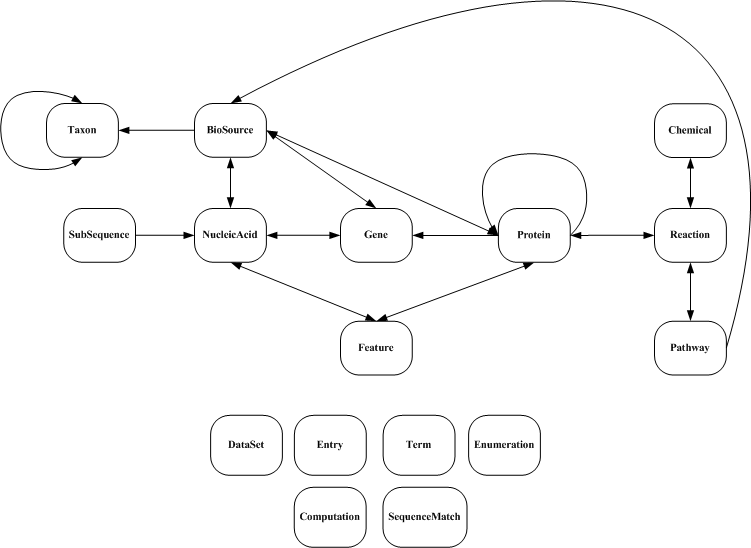
\includegraphics[width=5in]{figures/biowarehouse.png}
\caption[Original BioWarehouse schema.]{The main datatypes in the BioWarehouse schema, and the relationships between them.
\label{fig:biowarehouse}}
\end{figure}

The most recent contribution reported on their website is from August 2010 and includes the installation of the web based interface for mysql databases called myphpadmin. This highlights the lack of development that the project has had in the last 4 years. A similar situation has been observed in projects that follow the same warehousing strategy in bioinformatics. Most of them were published around the same period of time but have been inactive in recent years, or have broken links to the tool, for example, Atlas \cite{SHA2005} published in 2005, LCB\cite{AME2006} published in 2006 and M-Chips \cite{FEL2002} from 2002. From our research, the only active project on infrastructure of data warehousing for biological data is BioDWH, which is described below.

\paragraph{BioDWH}
The data warehouse for life science data integration known as BioDWH is a project developed at the Bielefeld University. BioDWH is a Java based project that developed an object-relational mapping using the library Hibernate to connect to the most common relational database management systems RDBMS (e.g. MySQL, Oracle, PostgreSQL) in order to create a centralised repository that integrates information from various biological databases \cite{TOP2008}.

BioDWH's main objective is to increase customisation of the data warehouse concept improving performance, scalability and having quality data up to date. As part of the project they have included some parsers to extract information from well-known available resources (e.g. UniProt, KEGG, OMIM, etc.). Figure ~\ref{fig:biodwh} presents the extensions to a general data warehouse design done in this project in order to define an architecture oriented to life sciences data.

\begin{figure}  
\centering
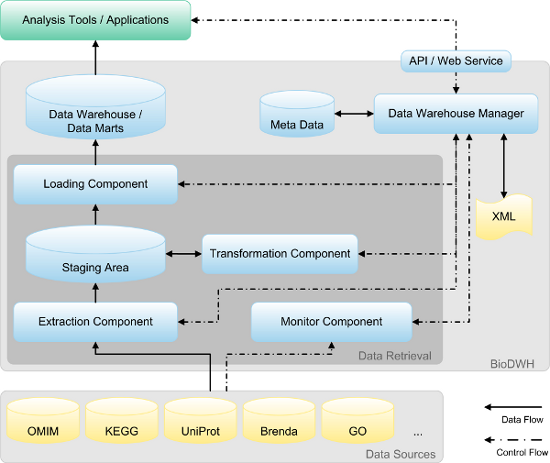
\includegraphics[width=4.5in]{figures/dwh_architecture.png}
\caption[BioDWH System Architecture.]{BioDWH System Architecture.
\label{fig:biodwh}}
\end{figure}

It is important to highlight the inclusion of a monitoring system that keeps track of the need for updates from the different sources. Instead of direct access to the RDBMS, BioDWH provides an API that can be queried remotely, and a Graphical User Interface that enables the configuration of the different components including monitors and parser along with the queuing and displaying of content.

Two projects have been reported in the literature that are using BioDWH: DAWIS-M.D. and VANESA. DAWIS-M.D. is oriented to metabolic data and integrates eleven different databases: BRENDA, EMBL, HPRD, KEGG, OMIM, SCOP, Transfac, Transpath, ENZYME, GO and UniProt \cite{HIP2010}. VANESA uses DAWIS-M.D. in order to access important information for the modelling of biological processes and systems as biological networks \cite{BRI2014}.

\paragraph{BioMart}
BioMart started by using the same principle as BioWarehouse, BioDWH and other projects of data warehousing in life science: ``\emph{to create one universal software system for biological data management and empower biologists with the ability to create complex, customised datasets}'' \cite{KAS2011}.

With this object in mind, BioMart has grown from an extension to the Ensembl website for data mining, to become an international effort for the integration of biological data. This has been achieved by first defining a general software infrastructure for further customisation, and then extending this architecture in order to support multi-database repositories as a data federation system, where all the entities use a predefined relational schema that is generic enough to support any kind of data.

\begin{figure}  
\centering
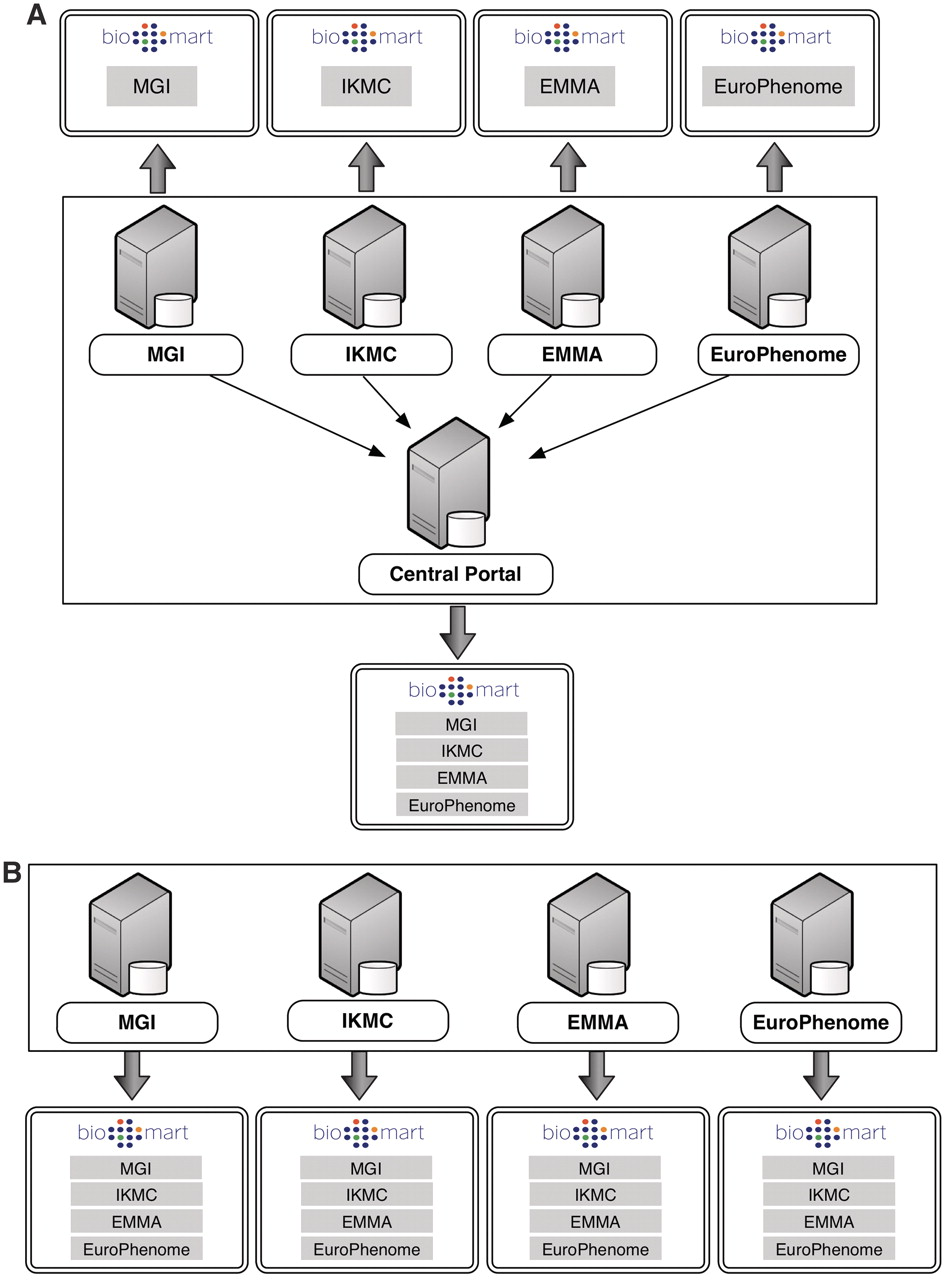
\includegraphics[width=5in]{figures/biomart.png}
\caption[Biomart Portal Architecture.]{Biomart Portal Architecture. The portal can be set either with a master/slave or with a peer-to-peer configuration.
\label{fig:biomart}}
\end{figure}

Given the inclusion of a multi-database paradigm, the BioMart team developed a server that provides access to a collection of sources called a BioMart Portal. Figure \ref{fig:biomart} shows the two possible configurations of the BioMart Portal. In configuration (a) each data source serves their own data and an independent server works as a central portal generating a unified view of the whole system. Alternatively, in configuration (b) all the data sources are treated as peers and they communicate with each other in order to be able to provide not only their own data, but also their peer's data.

BioMart includes a tool to automatically transform any 3rd form normalised database schema into the reverse-star scheme type used by this system. Once the dataset has been transformed, BioMart provides different view ports to it: Web-based Graphic Interface, Restful services and API connectors using Java \cite{KAS2011}.


\subsubsection{Federated databasing} 
This approach requires the agreement of multiple sources to follow a similar structure in order to allow a standard query over several instances. By dealing with smaller datasets than the data warehousing approach, the complexity of post-processing is simplified, however it requires that the providers deal with the extra work of maintaining their data as the federated database agreement establishes.

\paragraph{The HUPO Proteomics Standards Initiative}
The Proteomics Standards Initiative (PSI) is a collaborative initiative run by volunteers and coordinated as a work group of the HUman Proteome Organisation (HUPO), whose object is to define standards  to enable capture, comparison, exchange and verification of proteomics data. \cite{HER2006}. PSI is the result of a common effort from the interested parties in the proteomics domain.

This effort can be categorised into three major infrastructure elements: (1) A specification of the Minimum Information About a Proteomics Experiment (MIAPE), (2) data exchange formats that are compliant with MIAPE, and (3) the use of controlled vocabularies (CV) in order to ensure consistency on the data content. In this way the proposed standard can be stable while its content can evolve by updating the CV.

These recommendations are not intended to specify the methods and procedures for proteomics experiments, and should be seen as reporting guidelines.

This initiative has been growing for the last 10 years, and now its standards are widely adopted in the proteomics community. The proposed specifications cover different branches of the field, for instance the PSI-MI formats were defined to deal with Molecular interaction data, PSI-MS works on standards for mass spectrometry data and PSI-MOD focuses on protein modifications.

However even if all the parts follow the recommendations, a strategy to integrate this data is required. It is for this reason that the PSI common query interface (PSICQUIC) was created: a community standard that enables programmatic access to molecular-interaction data resources \cite{ARA2011}. This proposal includes a query language (MIQL) and an architecture to execute a query on distributed sources.

Figure \ref{fig:psicquic} shows the architecture of PSICQUIC. The idea is that several samples from an organism can be processed by different experiments, and their findings can be published in independent articles, which consequently can be stored in more than one interaction database. PSICQUIC proposes that the providers include an extra layer to access this information, which can be queried using MIQL and with responses following the PSI-MI formats. In this way a client can use a single query over multiple resources and create a unified image.

\begin{figure}  
\centering
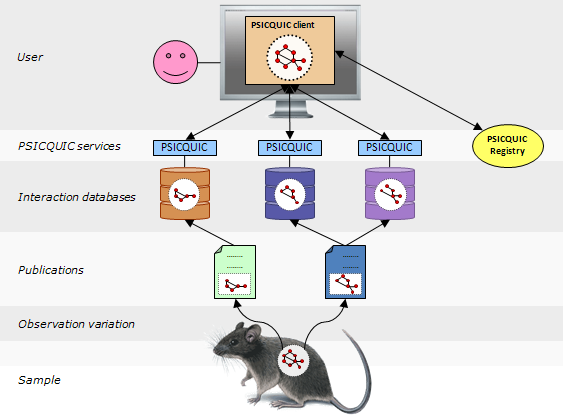
\includegraphics[width=4.5in]{figures/psicquic.png}
\caption[PSICQUIC Architecture.]{PSICQUIC Architecture.
\label{fig:psicquic}}
\end{figure}

The PSI group recognises the importance of providing software tools to promote the adoption of the proposed standards. The most recent implementation of the PSICQUIC web service was released when version 1.3 of the PSICQUIC specification was made public in 2013 \cite{DEL2013}. The providers of molecular interaction data are now asked to implement a number of methods in order to support both SOAP and REST web services. 

The web service methods will generally accept a MIQL query as input and generate an output in either PSI-XML or PSI-MITAB in its most recent versions. This implementation is based on the Apache Solr indexing software (\url{http://lucene.apache.org/solr/}), and is reflected in the constitution of MIQL, which is an extension of the Lucene query language used in Solr. This implementation is freely available for any provider who wishes to share their data to the PSI community.

Besides the server, PSICQUIC also provides client libraries to facilitate access to the information from three different programming languages: Java, Perl and Python. There are ready to use clients, for example the PSICQUIC View accessible from \url{http://www.ebi.ac.uk/Tools/webservices/psicquic/view/main.xhtml} or plugins for Cytoscape and the R Bioconductor package.

The last component of the PSICQUIC architecture is the registry, in which information about the available providers is stored as tags. This metadata can be used to query the registry as a RESTful service in order to facilitate the discovery of molecular-interaction data providers \cite{DEL2013}.


\subsubsection{Service oriented integration} 
The principle of service oriented integration is to have atomic components that offer a basic service. These services can then be connected in order to orchestrate the execution of a bigger task. Services can be data providers but can also be programs that execute specific functions.

The definition of a protocol for requests and responses to obtain data or execute services is the key to facilitate the connectivity between the software components. The two standards most widely used are SOAP (Simple Object Access Protocol) services and REST (REpresentational State Transfer) services, where the latter is gaining momentum because of its simplicity. However service oriented integration also requires a large commitment from providers in creating and maintaining the services, and also increasing and maintaining the specifications for the different domains.

Alternatively, the services can run on a local installation, which does not follow the principle of a unique remote resource executing a service to multiple consumers. Nonetheless, this option has been widely used in bioinformatics environments in order to have more control over the data and services offered.

\paragraph{Sequence Retrieval System}

The Sequence Retrieval System, better known in bioinformatics as SRS, was probably the most successful project before the introduction of Next Generation Sequencing (NGS) technologies, originally aimed at facilitating access to biological sequences databases \cite{ETZ1996}. It grew to become an integration system of both data retrieval and applications for data analysis.

SRS was developed following an object-oriented design with the strategy of taking advantage of raw text files, that were the \emph{de-facto} standard on molecular biology analysis. By dealing only with text files, SRS was getting faster retrieval speeds and saving storage space, mainly because data was neither stored nor parsed, only indexed \cite{ZDO2002}.

The  indexes obtained were linked via meta-data, offering the user access to the original source plus links to any conceptually related database. This was then presented in a web-based interface. The automatically created interface for different sources and applications can be complicated for beginners, however SRS provides ways to create customised interfaces.

Probably the most important instance of SRS was the one installed at the European Bioinformatics Institute (EBI), which was used to provide access to the major databases produced and maintained at the EBI. However by December 2013 the service was decommissioned as the service was considered redundant with the efforts to maintain multiple web services. Currently SRS technology is the property of Instem\textsuperscript{TM} and a list of available servers can be found at \url{http://bioblog.instem.com/download/srs-parser-and-software-downloads/public-srs-installations/}.

\paragraph{Taverna}
Taverna was originally conceived of as a tool for non expert programmers to design, execute and share workflows of web services \cite{HUL2006}. Bioinformatics web services can be a way of providing the available data in a data source (e.g. the PSI services), but traditionally, web services are seen as a remote software component that receives some input data, processes it and generates output data. The main advantage of using web services  is that most of the processing load is delegated to the service provider, allowing small groups to run high throughput analysis in remote but powerful machines.

Taverna is a tool that allows the user to create ``recipes'' of combined web services or pre-composed workflows to execute a higher level computational experiment. The Taverna workbench is a graphical interface that allows the design of workflow, that can be executed either on the same workbench or in independent runner tools such as the Taverna command-line application, the Taverna server or the Taverna lite installation.

By 2013 the Taverna project was reported to have access to over 8000 service operations \cite{WOL2013}. With such a large number of resources, there is a necessity to make them searchable. This is the goal of the BioCatalogue: a registry for web services where both REST and SOAP services can be discovered using their metadata. Taverna supports searching on the BioCatalogue and inclusion of a chosen web service through its workbench tool.

It is often necessary to do intermediate processing to be able to connect two services, where for example one produces the data that is required for the second but in a different format. Taverna provides a set of what they call ``shim'' services to cater for this need. Other types of services that are supported by Taverna are local, grid and cloud services, access to BioMart, R-Scripts and distributed command-line scripts.

The number of ready-to-use workflows have grown in recent years, which is ideal for researchers that need a starting point for their experiments. However this number is so large that finding the right pipeline for an analysis is not an easy task. For this reason MyExperiment was developed, it not only supports Taverna workflows but also other systems such as Galaxy (discussed below). To run a workflow found in the MyExperiment repository in Taverna is as easy as copying the URL into the workbench importer, adjusting the parameters and pressing ``run'' \cite{WOL2013}.

\paragraph{Galaxy}
Starting as a project to integrate genomic sequences, their alignments and functional annotations, Galaxy has evolved rapidly in less than 10 years to the point of offering a complete web-based framework that aims to enable reproducibility, accessibility and transparency for computational biology experiments \cite{GIA2005, GOE2010}.

First versions of Galaxy were written in a combination of C for the core components and Perl for the user interface, promising the possibility of adding new tools thanks to its architecture. Nowadays the project has been rewritten in Python and follows an open source strategy with over a hundred commits per month on its public repository (\url{https://bitbucket.org/galaxy/galaxy-central/overview}), and the extensibility promise has been fulfilled to the point of asserting that Galaxy supports any tool that can be run in the command line.

This feature marks the greatest difference between Galaxy and Taverna, because the latter has web services as its basic workflow unit while Galaxy is used to compose workflows using command-line tools.

Galaxy's main goal is to provide a tool where experiments can be reproduced easily and reliably; and Galaxy's authors consider that because it is in the nature of web services to be hosted by remote and probably unknown service providers, the reliability is compromised, and therefore web services are not natively included in Galaxy.

Despite the fact that the origin of Galaxy did not explicitly include the execution of workflows as its core functionality, Galaxy's detailed history of task executions has evolved and currently it offers all the advantages of a modern workflow execution suite.

The addition of metadata to both workflows and tools, and its publication by the means of Galaxy Pages makes the project easier to share. A well annotated workflow can be understood better when its documentation goes beyond the sequence of tools that have been connected, and includes the biological meaning of such executions.

There is an instance of Galaxy publicly hosted at \url{https://usegalaxy.org/} where a subset of features can be explored by anonymous users and the rest of the functionalities become available after free registration. This public tool includes hundreds of tools for getting data, processing it and visualising it. If however, a project has particular requirements such as including non-public tools, Galaxy can be installed as a local server and the tools can be added to that instance \cite{GIA2005, GOE2010}.


\subsubsection{Semantic integration} 
The main methodology under semantic integration is to structure the data using semantic web standards (e.g. RDF, OWL) in order to make it ``machine-readable'' and be able to deduce meaningful associations. The conversion of the data into RDF files might not be a trivial endeavour, and it has similar problems to the ones mentioned above because it usually implies maintaining copies of the information in a separate format. 

\paragraph{BioMOBY}
BioMoby is one of the attempts to bring the promises of the semantic web into bioinformatics, proposing an architecture for the discovery and distribution of data though web services using multiple proposed standards of the World Wide Web Consortium (W3C) such as the Simple Object Access Protocol (SOAP). Its main goal is to provide access to biological data and services with a common format among the different sources \cite{WIL2002}.

The strategy of BioMoby is to define a minimalistic entity to describe the data in such a way that different types of data can use the same schema.
This structure has been called the MOBY object, and is composed of three values: the MOBY object type (e,g. Sequence), a namespace identifier (e.g. Genbank/AC) and an accession number (e.g. AY070397.1). MOBy object types are defined using XML Schemas (XSD) reflecting a hierarchical relationship between them.

An important component of the BioMoby ecosystem is MOBY Central: a server that contains information not only about available services, but also their association with MOBY objects for input and output. With this information a MOBY client can suggest paths to follow depending on the current type of your data. Moreover, the intrinsic semantics of this approach is the ideal environment in which to create cohesive workflows.

\begin{figure}  
\centering
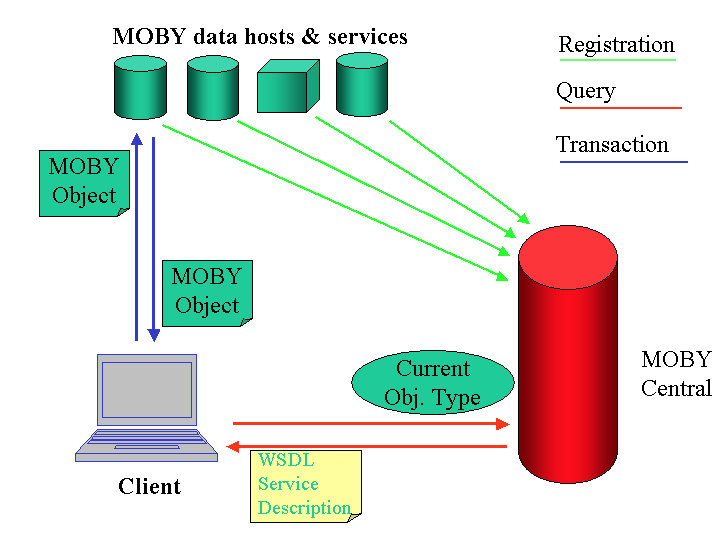
\includegraphics[width=4in]{figures/MOBY_Overview.png}
\caption[BioMoby Overview.]{BioMoby Overview.
\label{fig:biomoby}}
\end{figure}

Figure \ref{fig:biomoby} shows the adaptation done by BioMOBY to the classic web services architecture: once all services have registered with MOBY central, a client can query it to find out which services can be used with the current MOBY Object. Besides the discovery feature, the central repository has the capability of generating a Web Service Description Language (WSDL) document that can be used with the corresponding service, where both input and output are MOBY Objects.

A more recent iteration of the development of MOBY was described in \cite{VAN2009}: Moby-2. The objectives of the project have been extended and its focus on semantic web technologies is stronger: MOBY Central will take the form of a Resource Description Framework (RDF) triple store and will support the functionalities of a SPARQL endpoint. These changes were done with the objective of allowing semantic queries over multiple sources. The project was reported in \cite{VAN2009} as a prototype, but promised to contribute towards a distributed, machine-readable semantic web of life science data.

\paragraph{Bio2RDF}
A simplified view of the Semantic Web can be defined as a network where the nodes represent any entity that can receive a name and the edges correspond to the characteristics used to describe the relationships between the nodes. The RDF format is an XML-based language that describes this relationships as a set called a ``triple'' that contains subject, predicate and object.

Bio2RDF uses RDF documents to be able to create a knowledge base that takes advantage of existing developments on the semantic web to build a mashup of data in the bioinformatics domain.  \cite{BEL2008}.

One of the main objectives of Bio2RDF is to extract information from the most important bioinformatic databases, transform its content into RDF, and load it into a triple-store. It is within a triple-store that discovery of new knowledge occurs through recombination analysis of the loaded data. In this sense, Bio2RDF follows the approach of a data warehouse of semantic data.

As part of the project, a set of software tools that convert different datasets into RDF called ``Rdfizers'' were created. There is one rdfizer for each source, however they can be grouped in three types depending on the origin of the data: XML to RDF, SQL to RDF, and text file to RDF. For large scale resources such as UniProt or PubMed where programmatic access to the data is provided, the rdfizer works on-demand, which means that it only stores some of the data for cache purposes and the RDF files are created on the fly. Any other source gets copied into the centralised repository in order to offer quick responses.

The Bio2RDF approach can be summarised in three steps: (1) build a list of namespaces for data providers, (2) analyse a data source to represent it in an RDF model and (3) develop rdfizer to convert the information. The resulting dataset is sorted in the triple-store in order to connect it all together.

Bio2RDF used an extended version of Sesame as the triple-store and on its 2nd release was changed to Virtuoso in order to offer better support to SPARQL, which is the most widely used query language for semantic web data. Bio2RDF makes use of other tools such as Protégé: an ontology editor, the Piggy Bank: a semantic browser for Firefox and Welkin: a RDF graph visualiser; all of which are well known projects in the semantic web community \cite{BEL2008}.

\paragraph{SADI}
The Semantic Automated Discovery and Integration (SADI) project has its roots in the lessons learned from BioMoby, particularly  Moby-2. However, unlike BioMoby, SADI is not a data typing system. The goals of SADI are centred on the proposal of patterns and best practices of how to use web services connected through semantic web technologies to enable the creation of interoperable and integrative bioinformatics software. \cite{WIL2011}.

The biggest change introduced by SADI in respect to SOAP web services is to replace the defined languages for communication between the web services parts (e.g. WSDL, XML Schema,UDDI) with structured versions of semantic web languages: RDF and OWL. The authors go as far as to say that XML Schema is the problem causing the failure of most previous interoperability architectures.

A description of an interaction with a SADI service is as follows: A client requests the service description via HTTP GET, and the server responds with a document containing references to OWL classes describing input and output datatypes for the service. The client uses data formatted in RDF that follows the received description to submit an HTTP POST request, which is captured by the server, which in turn uses it to execute the service and generate a response in RDF format.

The adoption of HTTP methods for communication follows the positive reception of ``RESTful'' Architectures. SADI does not claim to follow a RESTful architecture, but it sees the potential of it and uses some of its principles. This is partially a response to the general dislike of the SOAP architecture within the bioinformatics community.

The use of a good ontology to connect services is seen in SADI as the key component to meaningful interoperability, where the interaction between servers is guided by biological knowledge and not only by technicalities such as format and availability \cite{WIL2011}.

As part of the project, software components have been developed in order to facilitate the adoption of the recommendations including plugins for Taverna and Protegé, and a  prototype of all the components (i.e. Servers and clients) is available at \url{http://biordf.net/cardioSHARE/}.


\paragraph{BioPAX}
The Biological PAthway eXchange (BioPAX ) is a community driven effort to develop a standard language to facilitate knowledge representation of biological pathways at molecular and cellular level in order to enable the systematic collection, distribution and integration of pathway data from heterogeneous sources \cite{DEM2010}.

BioPAX also takes input from the semantic web community. In this case OWL is used to define an ontology to describe pathway information, which can be used to interconnect the multiple resources in this domain. BioPax has, among others, been used to describe (1) metabolic pathways, following the abstraction: ``enzyme, substrate, product''; (2) signalling pathways for biochemical reactions, binding, and catalysis events; (3) gene regulatory networks involving transcription and translation events and its control; (4) protein-protein interactions and protein-DNA interactions; and (5) genetic interactions i.e. when the phenotype of perturbing two genes is different from the expected known phenotype of the perturbation of each isolated gene.

The BioPAX ontology is the result of ongoing periodical workshops that involve the different stakeholders in the biological pathways field. Incremental versions of the agreement, also called levels, have been developed with the concept that newer levels can replace older ones. Currently the highest  is level 3.

A tool set called Paxtools has been developed as part of the project. The main features of this software include an implementation of the specification as a software model, the support of OWL properties, a syntactic validator, transformation scripts between levels, import and export to other formats. Thanks to these features, Paxtools can and has been used as the framework to develop other tools \cite{DEM2010}.

\subsubsection{Wiki-based integration} 
It is a cooperative effort where the community inputs information in an open and unstructured way, which can reach a highly reliable status as has been shown in the case of wikipedia. It is however completely dependent on the adoption of the community, and also given the unstructured nature of the data, is hard to manipulate for automatic analysis.

\paragraph{WikiPathways}
Following the success of wikipedia, where any user can contribute to an article and the tasks of editing and curation are community based; WikiPathways has been developed with the objective of providing an open platform to deposit, share and curate biological knowledge in the form of pathway diagrams \cite{KEL2012}.

Biological pathways are representations of the compiled knowledge of biological units and their relationships. Pathways are vital to understanding genes and proteins in terms of larger systems and processes of any organism. The challenges of gathering knowledge about biological pathways are particularly hard: (1) pathway information is not measurable and can't be obtained from a single experiment, (2) many different representations and methods have already been used, and (3)  representations are usually saved as static images, which are far from ideal for computation and integration \cite{PIC2008}.

Looking to tackle these challenges and inspired by how science has been gaining a more open approach by means of open journals, public databases, data exchanges formats, ontologies and free software; WikiPathways provides a web based framework where the community can not only take information but also give back.

In WikiPathways, each pathway has a dedicated page that summarises the existing information around the specific biological mechanism including its diagram, description, links, related genes and proteins, and relevant literature references. The pathway is displayed using an interactive viewer that supports navigation and live highlighting. Registered users can also use the viewer to improve a pathway, and all the information can be exported in suitable formats such as the BioPAX standard.

A subset of the functions of the web-site can be programatically accessed via web services.

The metadata associated with the pathway serves the purpose of making it searchable, but most importantly makes it easy to integrate with other resources because it follows an ontology that as a side effect can be used to organise the created pathways in a hierarchical fashion.

Nonetheless it is clear to the authors that the tools and developments only assist in the community building process and its in the growth of the community itself that the future of WikiProteins is held \cite{KEL2012}.

\paragraph{WikiGenes}
In contrast to what its name suggests, WIkiGenes is not exclusively about genes; its scope goes beyond genes and aims to construct a knowledge base of biological information including chemical compounds, proteins, organisms, pathologies and of course genes. 

Similarly to WikiPathways, WikiGenes applies a strategy based on the wiki model, however in \cite{HOF2008} the author argues that given that the wiki model was not created taking into account the demands of the science ecosystem, it requires significant technical innovation. In particular, current wiki alternatives do not consider the current scientific publications paradigm, and the relevance of authorship. 

The advantages of having a continuously updated article on each topic are obvious, however the effort from contributing scientists to reach this goal is quite considerable and the personal benefits of such efforts are not very clear. Traditional scientific publications recognise the efforts of a contributor by clearly stating its authorship, which in today's academic world might get reflected in employment, grants and ultimately in the privilege of being a scientist.

WikiGenes proposes a system where every word of a document can be linked to its author in order to provide him/her with his/her due recognition. Such a document is reviewed by its readers as in the wiki model, however WikiGenes includes a reputation system that can be used to solve disagreements between authors and avoid vandalism.

More than a hundred thousand generated articles on several biomedical concepts have been included in WikiGenes. It is clear that the quality of these articles is not the best, but it serves as a starting point for interested authors \cite{HOF2008}.


\subsection{The Distributed Annotation System}
%\footnote{Most of the text in this section was originally included in the lead author's MSc dissertation\cite{SAL2010} and edited here to update it where necessary.}
The Distributed Annotation System (DAS) \cite{DOW2001} makes use of a widely-adopted standard communication protocol. It is motivated by the idea of maintaining a federated system; a logical association of independent sources distributed over multiple sites, which provide a single, integrated, coherent view of all resources in the federation. This architecture makes several distinct physical data sources appear as one logical data source to end-users. 

\begin{figure}  
\centering
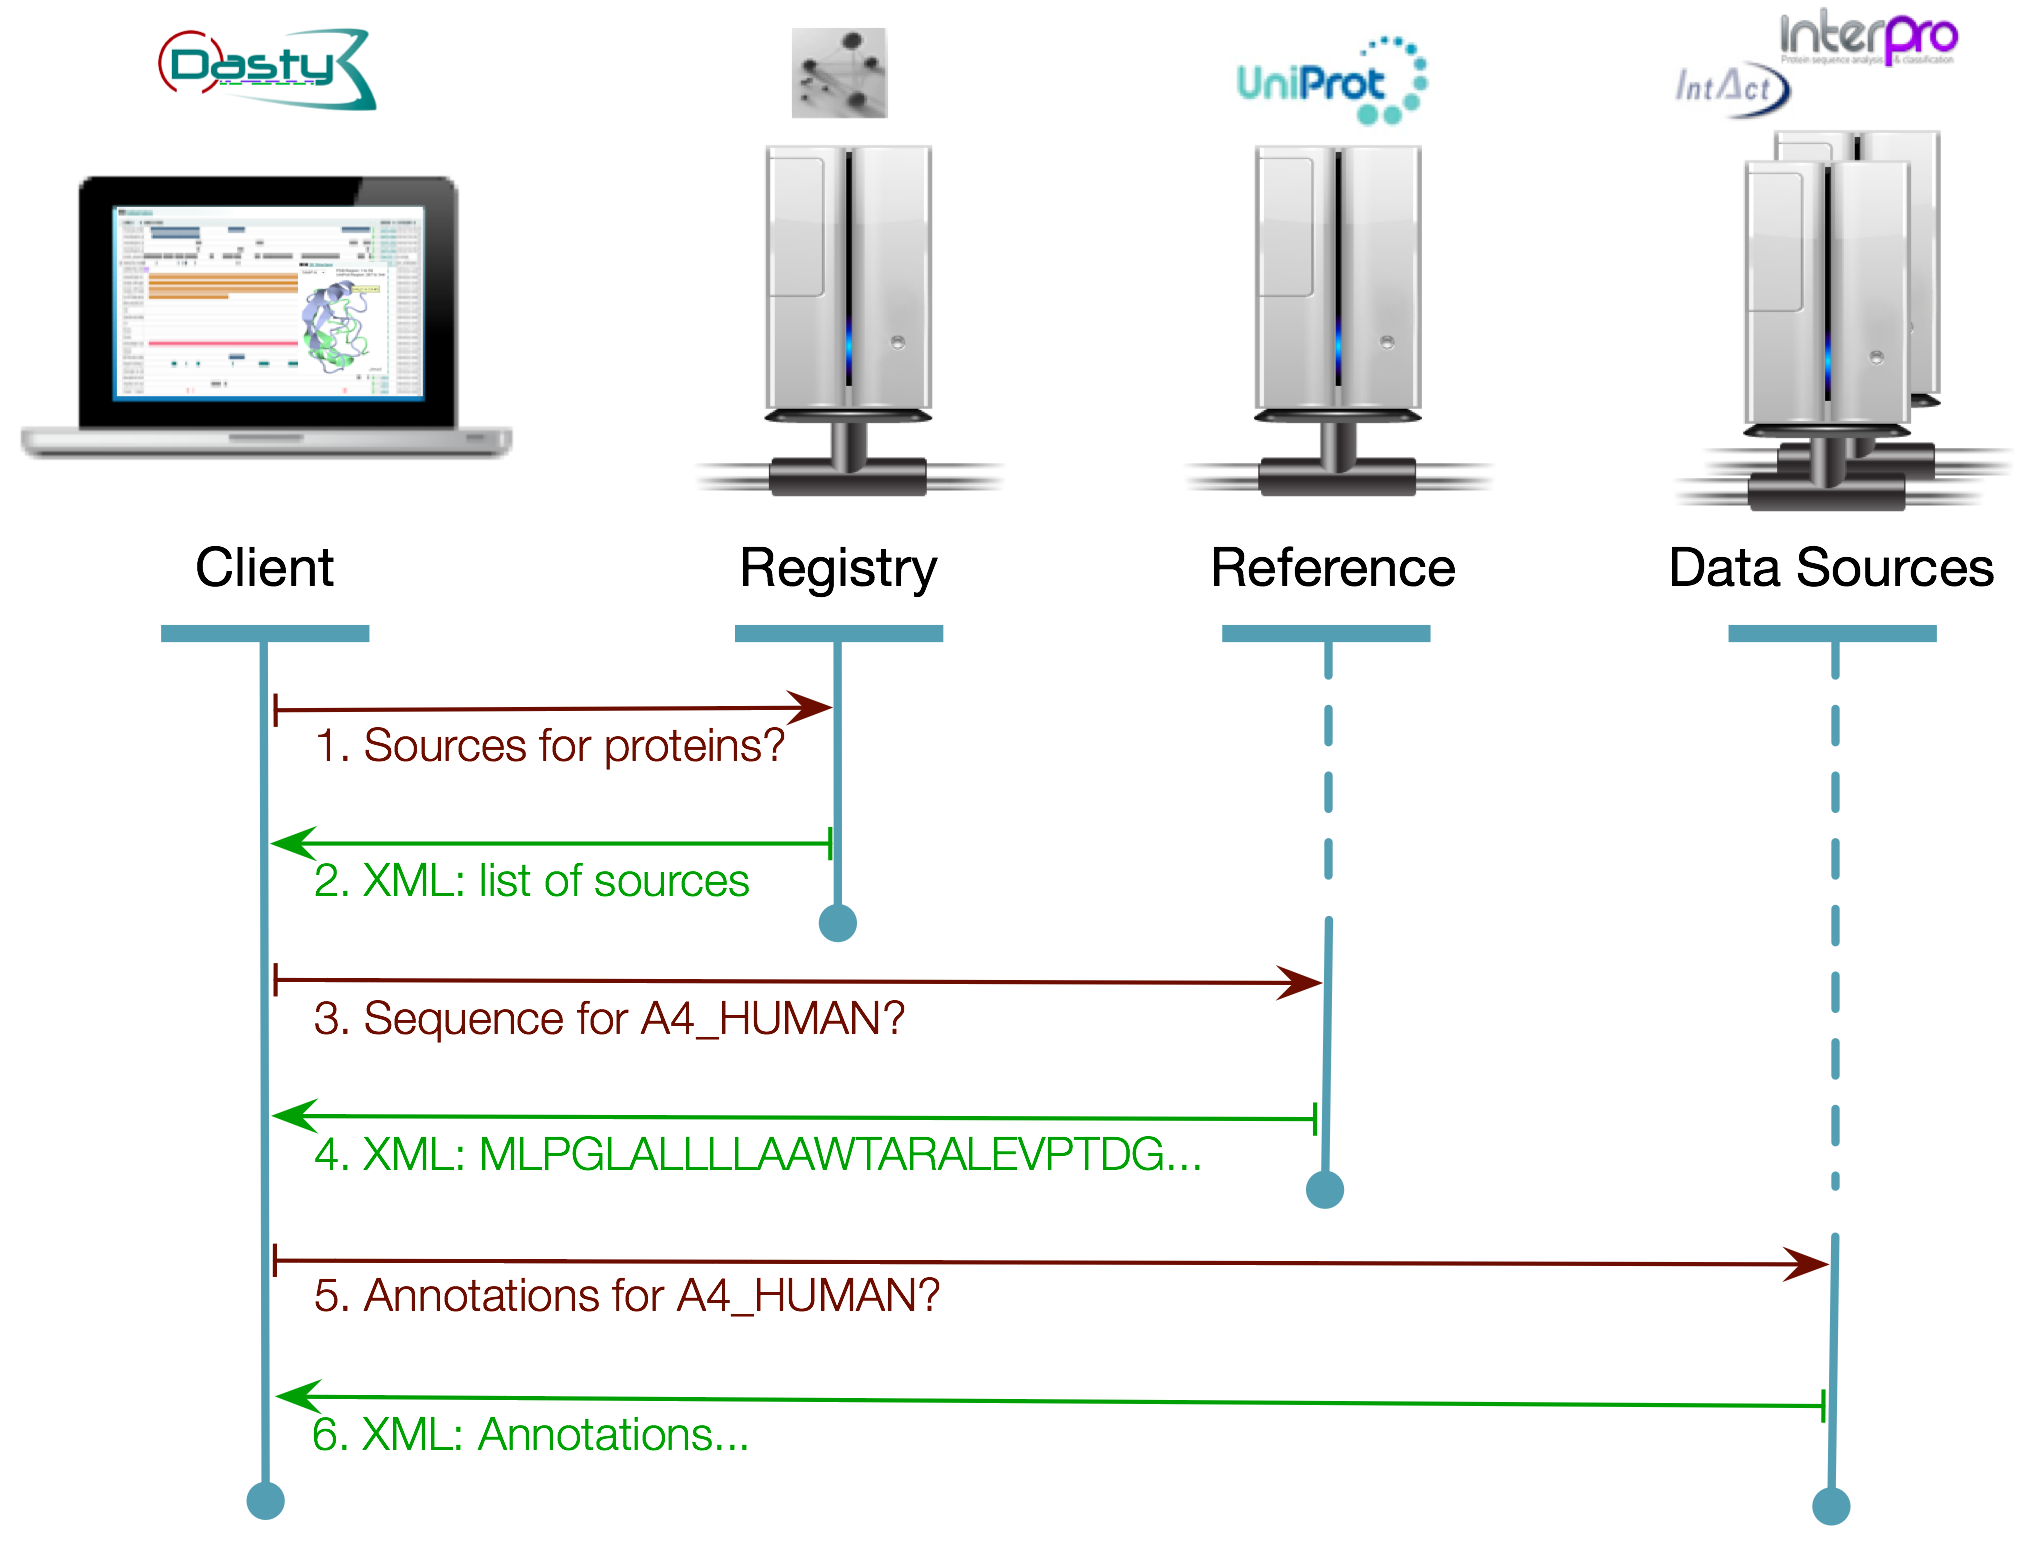
\includegraphics[width=5in]{figures/DAS.png}
\caption[DAS Flow of Information.]{Flow of information in a standard query in the Distributed Annotating System.
\label{fig:das}}
\end{figure}

A regular flow of information in DAS is shown in Figure \ref{fig:das}. The DAS client requests information about a protein that can be specified by its accession or identifier. The client then communicates with the DAS registry in order to retrieve a list of available sources providing information about that biological product. Once the client has retrieved this list, it proceeds to query the DAS reference source, i.e. a DAS source providing the sequence or structure of each molecule that it describes -- UniProt in the case of proteins. The DAS reference source supplies not only the sequence but also meta-data such as the version. Thus clients can ascertain which retrieved annotations correspond to the original request. At this point, the client retrieves features, i.e. annotations, from the available DAS sources. These annotations may be applicable to specific subsections of the sequence (e.g. the location of active sites or observed peptides) or may be applicable to the entire sequence (e.g. related publications or taxonomy). Finally, the client organises and displays the annotations \cite{SAL2010}. 

All these interactions follow an adaptation of the REST protocol for web services \cite{PRL2007} .

\subsubsection{DAS Protocol}
\label{ssec:DASprotocol}
The DAS specification consists of a set of rules which define a standard communication method between the different components of the system. DAS is Web-based and makes extensive use of three widely-adopted standards: the Unified Resource Locator URL, the HyperText Transfer Protocol HTTP and the eXtended Markup Language XML. All communication occurs through HTTP; the requests are URLs that specify the resource that the client is interested in, and the responses are both HTTP codes and XML documents. The details of what constitutes a valid URL, and the XML structure, are contained in the DAS specification.

By the time the first paper about DAS was published \cite{DOW2001}, the DAS protocol was version 1.01, and the main characteristics, such as the \emph{features} and \emph{dna} commands of DAS, were present in that version. From that point, several versions were released with minimal changes. These subsequent versions mostly just polished details to make the protocol stable and useful. The last official release of DAS was Version 1.53 on March 21 of 2002. This was the official version for several years, but in 2006 a new version appeared (version 1.53E) incorporating several new developments. These included an extension to serve new data types and an ontology for protein features \cite{JEN2008}. The E in the version number is for Extended, which essentially describes the purpose of this version, because it keeps most of the features present in 1.53 but extends these to provide some new capabilities.

In November 2007, a project that aimed to define a completely new specification for the DAS protocol was concluded. The new specification was called DAS 2.0 (\url{http://biodas.org/documents/das2/das2\_protocol.html}) and it contained a redefinition of the protocol for the capabilities that DAS had in its previous versions (1.0, 1.53). It also defined new features which allowed for the use of the protocol in a more extensive way. A controversial topic in the DAS community was whether or not the DAS2.0 protocol should be adopted. This specification contains several improvements to the DAS protocol, but given the drastic changes in the format, amongst other reasons, most of the sources decided to continue using DAS1.53 or 1.53E. After the 2009 DAS workshop, it was generally agreed that most of the useful additional features that 2.0 provides would shortly be implemented in DAS 1.6E and its subsequent incarnations. As a result, DAS2.0 is now considered by many to be redundant. Figure \ref{fig:dasevolution} represents the evolution between the various version of DAS, and serves as a comparison between DAS 2.0 and 1.53E/1.6E in terms of number of sources, which is a good indicator of its adoption.

\begin{figure}  
\centering
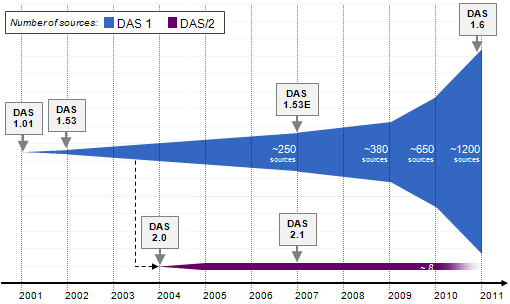
\includegraphics[width=4in]{figures/DasEvolution2.PNG}
\caption[DAS Evolution.]{DAS Evolution.
\label{fig:dasevolution}}
\end{figure}

Version 1.53 of DAS defines the element \emph{FEATURE} as the annotation itself, and it is contained in the element \emph{SEGMENT} indicating that a feature annotates a specific segment, where a segment is a biological residue (or part of it), such as, proteins, genes, chromosomes, etc.

In the scope of proteins, annotations can indicate information about the structure (known formations of amino acids such as helices or sheets), interaction zones (with other proteins or regions of the same protein), phenotype (for example a known relation of part of the protein with a disease), etc. 

An effort to group and organize all the types of annotations has been made: the Biosapiens Ontology contains, in a hierarchical structure, the types of annotations that can be used. As with any ontology, the information is not complete and periodic releases are made trying to establish a set of types as efficiently as possible.  \emph{TYPE} is probably the most important element included in a \emph{FEATURE}. The use of the Ontology is highly recommended but is not mandatory, in order to comply with older releases. 

The use of a second ontology (Evidence Code) is also recommended in the attribute \emph{category} to express the method through which such an annotation was acquired, for instance by experiment, by \emph{in-silico} analysis, etc.

Relevant information for proteins included in the element \emph{FEATURE} is registered in:

\begin{itemize}
\setlength\itemsep{-0.3em}
 \item \emph{id:} A source can not have two features with the same id.
 \item \emph{label:} A human readable label for the feature
 \item \emph{START} and \emph{STOP}: Indicating the specific position to be annotated. If both are equal to zero, it means that the annotation applies to the whole segment (i.e. \emph{Non-positional feature})
 \item \emph{LINK}: To indicate a URL where more information about this annotation can be found.
 \item \emph{NOTE}: Space where the annotator can put any extra comment about the annotation.
\end{itemize}

Other elements and attributes are more oriented to other kinds of biological data, for instance the \emph{ORIENTATION} element is useful for genes, to indicate if the annotation follows the direction 3' or 5', however proteins do not have an orientation.

DAS can be seen as having a \emph{``Dumb server -- Smart Client''} architecture where most of the hard work is executed in the client. Nonetheless, several independent projects have contributed to both clients and servers. 

Under the DAS terminology, servers and sources represent two different concepts. A \emph{DAS source} provides data for one \emph{Coordinate system} (\url{http://www.dasregistry.org/help_coordsys.jsp}), i.e. a unique 4-tuple \emph{(Authority, Version, Type, Organism)}, e.g. (Ensmbl, 51, Chromosome, Homo Sapiens). On the other hand a \emph{DAS server} is the software that facilitates the publishing of DAS sources.

Each DAS source can support several capabilities, which means it is able to respond to an HTTP request that gets interpreted as a DAS command (e.g. sequence, features) with a document that follows the specification. DAS servers are pieces of software that implement the common tasks of this process, for example handling the HTTP requests, providing a logical model for DAS or encoding the model into a document.

The two most representative implementations of a DAS server are Pro-server \cite{FIN2007} and MyDas \cite{SAL2012}. Both have been updated to support the latest version of the specification (i.e. 1.6E) and their feature sets are similar. Probably the biggest factor in choosing between these two implementations is the preference for a particular programming language: Perl for Pro-server and Java for MyDas. An extended description of MyDas can be found in the section \ref{section:mydas}, including the contributions to MyDas as part of this PhD project.

On the other side of the spectrum, the DAS clients have the task of providing a unified view of multiple sources. Most of the DAS clients centered their efforts on a particular DAS type, such as proteins (e.g. DASher \cite{MES2009}), chromosome (e.g. Ensembl viewer \cite{FLI2011}) and genomes (e.g. Dalliance \cite{DOW2011}), where others such SPICE provide a way to navigate between multiple DAS domains. For instance, it is possible in SPICE to start on a chromosome view, zoom-in into a gene region, select the expressed protein of the gene and visualise its 3D structure, all in the same Java Web-start window \cite{PRL2005}.

Dasty2 is a Web client that also supports the interaction between protein data and its 3D structure, but its current version doesn't support direct manipulation of genomic data \cite{JIM2008}. A refactoring of Dasty was executed during 2010 and is explained in detail in section \ref{section:dasty}, including our contribution to the effort of developing Dasty3 \cite{VIL2011}. 

\subsection{Discussion}
Besides the primary data from \emph{in-vitro} experiments, there are hundreds of secondary sources consolidating data that results from \emph{in-silico} analysis. All the projects mentioned contribute in different ways to the creation of a pool of knowledge where both primary and secondary sources are available to the researchers.

Some of these projects started when a problem was detected while trying to compile the generated data of a particular community (e.g. BioPAX); while others have studied an existing technology such as data warehouses, web services or semantic web and proposed adaptations to it for bioinformatics needs (e.g. Biowarehouse, BioMoby). Some approaches are on the protocol and specification level (e.g. SADI) while others take existing specifications and generate the tools to facilitate their implementations (e.g. BioRDF). There are projects that take existing software and adapt it to bioinformatics (e.g. WikiPathways) and others develop completely new software (e.g BioMart, Taverna). Some focus on the integration of the data (e.g. BioMart) and others on the interconnections between components (e.g. Galaxy). Some focuses on the tools (e.g. SRS) and others on the results and their publications (e.g. WikiGenes). 

Despite their origin, methods, technologies or approaches; all of these projects have in common the need for a strong community that supports its development, maintenance and use. We chose DAS as the base technology on which our contributions will be focused because when we started the project, it had a growing community as seen in figure \ref{fig:dasevolution}. It was based on existing and consolidated technologies such as the HTTP protocol and REST services, and it had the support of big entities and projects, such as the EBI and Ensembl. A description of the specifications and software components developed as part of this PhD project can be found in chapter \ref{section:integration} of this document.

\newpage
\section{Visualization}
The field of visualization aims to represent data in a way that non evident features became visible. The developed techniques in this search varies from simple ones (e.g. histograms) to very elaborated (e.g. environments just visible using 3D virtual reality rooms).

The uses of visualization techniques are as diverse as fields are in the world, from weather forecast in the news to the analysis of the captured data in the Large Hadron Collider. In the field of our interest: bioinformatics, the use of visualization methods is also abundant and sub-fields such as genomics, proteomics, population variance, etc. have plenty of examples were different techniques have been implemented with the purpose of making sense of biological data via visual representations.

%The section below is a review of the most relevant existing tools and techniques in different bioinformatics fields.

%\subsection{Visualization tools in Bioinformatics}
The most representatives visualization techniques used in bioinformatics can be categorised in three groups: charts, networks and hierarchies. Charts are graphical representations were n-dimensional data is mapped or aggregated into a space, for example scatter plots, bar graphs, pie charts, etc. Networks are structures were some components are connected to an arbitrary number of other components, normally using a node-link metaphor were the components are represented by nodes and the connections are lines in between them. Lastly, the hierarchies are another type of connection showing when an item is part of another, or using graph theory terminology, a node can be the parent of another; the diverse representations of trees can be used for this type of data, for example, node-link trees and space filling diagrams \cite{WAN2014}. 

\begin{figure}  
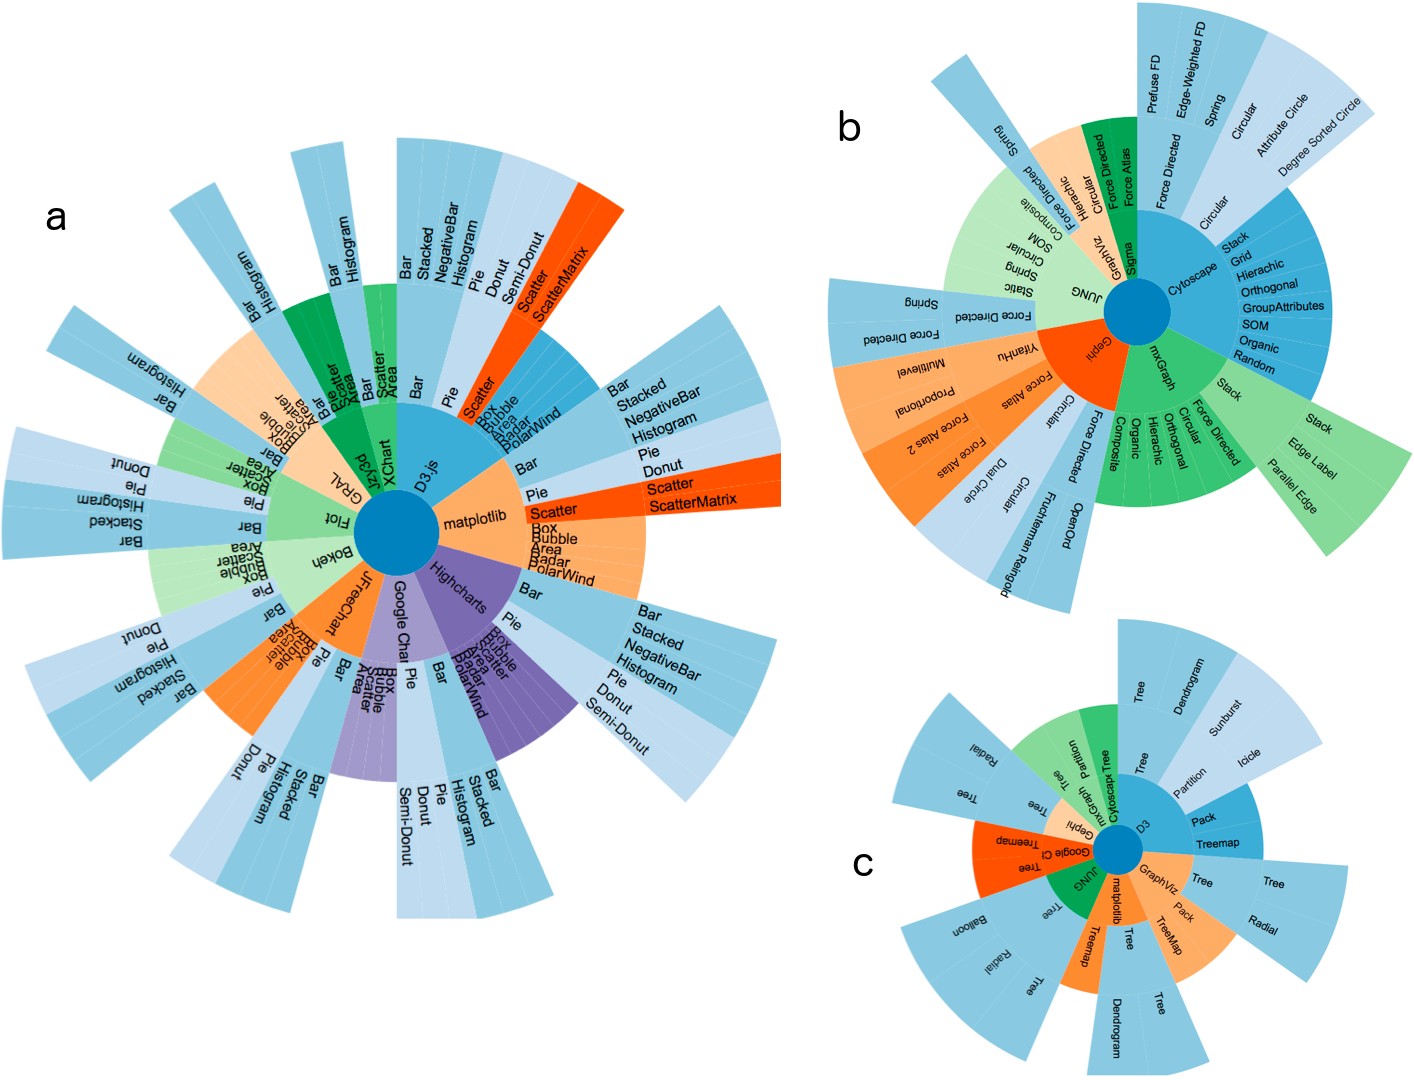
\includegraphics[height=6in,angle=90]{figures/vis_libs.png}
\caption[Comparison of feature of selected visualisation libraries.]{Comparison of feature of selected visualisation libraries.
\label{fig:vis_libs}}
\end{figure}

Figure \ref{fig:vis_libs} shows a a comparison of several libraries that have been used in bioinformatics research; The libraries in (a) include capabilities to represent charts, while (b) and (c) are show similar graphics for libraries that support network and hierarchical representations respectively. It is noticeable than several libraries are in the 3 graphics making evident its multi-purpose nature, where many visualisation techniques are embedded in the same package.

A recurrent challenge when visualising data is to match the most appropriate combination of techniques to the nature of the data, optimising the features of the visualization (e.g. location, colour, size or shape) in order to highlight a biological characteristic (e.g. genomic position, functional class, expression level or organism). Or as stated in \cite{GEH2010} ``\emph{The challenge is to create clear, meaningful and integrated visualizations that give biological insight, without being overwhelmed by the intrinsic complexity of the data}''.

A variety of projects in different subdomains of bioinformatics have been presenting alternatives according to the needs of each case. The sections below describe some of the most illustrative projects, grouped by some well known bioinformatics domains.

\subsection{Genomics}
Genomics is arguably the subfield that produces the most abundant, basic and yet relevant type of data in molecular biology research. Advances in the methods for extracting DNA, RNA and other biological products have grown dramatically in the recent years. For example sequencing projects have accelerate from the immense effort required to the get the human genome sequence in which took over a decade to put together approximately 3.3 billion base-pairs \emph{pb} to been able to extract over a billion of short reads(i.e. individual sequences of approximately 100bp) in days or even hours with some of the new technologies known as Next Generation Sequencing NGS.

This is quite an unfair comparison because the number of reads produced in NGS still requires lots of processing in order to assembly a genome (but not in the order of years). Moreover, none of the NGS technologies would it be possible without the learnings and findings of the human genome project, nonetheless the comparison is still valid in order to reflect the rapid growth on the methods to sequence DNA.

Visualizations have played an important role in the different stages of genomic analysis. In \cite{NIE2010} the authors have identified three tasks in genomic research were visualizations have been widely used: (i) supporting the sequencing process, (ii) browsing annotations in the context of a reference genome, and (iii) comparing sequences from different organisms and/or individuals.

\subsubsection{Sequencing Process}
Despite all the progress on sequencing techniques the process is not perfect and requires visual inspection in order to interpret and validate automated outputs to compose sequences, chromosomes and ultimately genomes. It is a common strategy to associate quality scores QS to each of the nucleic bases that result from a sequencing experiment. The QS is proportional to the number of agreeing reads that cover a base, for example the QS on a given position X would be really low if half the reads covering X indicate a G and the rest point to a T, it would be similarly low if only few reads cover that area or if the bases are not clearly distinguish in the reads. In contrast, if many reads are covering an area and all of them coincide that position X is an A, the score in that position should be really high.

Several tools have been developed in order to take advantage of this information, aligning the reads and representing the scores in multiple ways, for example histograms or heat maps, making easier the task of identifying regions of low coverture and discover errors in the automatic consensus sequence. This type of tools is highly dependent on the used technology, for instance, there are no raw read traces(only images) in some of the NGS techniques, and therefore a detailed alignment is prohibited because of the elevated computational cost.

Some of the read alignment viewer tools go beyond the display functionalities to offer edition of the assembly in order to complement the automatic outcome and to annotate relevant part on the sequence (e.g. genes, promotors, etc).

HawkEye was one of the pioneer tools that offered some of the feature discussed above mainly focused to assist in the detection and correction of assembly errors for whole-genome shotgun projects.  \cite{SCH2007}. 

This stand-alone tool offers a Top-Down strategy to analyse an automatic assembled genome. Figure \ref{fig:hawkeye} presents the three main views included in Hawkeye: 
\begin{description}
\item[(a) The launch pad] is the first screen presented to the user when a draft genome has been loaded, it acts as a global overview by displaying summary assembly statistics in the form of two N-Plots (i.e. A bar graph where each bar is a contain, its height represents the length of the contain in pb, and the width its length in percentage of the genome size.
\item[(b) The Scaffold View] represents the current scaffold as a linear ordering of connected contigs, with the assembly features displayed below. the first two tracks are heat map plots to easily visualise the insert and read depth of coverage. the view allows zooming and panning in order to navigate through the assembly.
\item[(c) The Contig View] follows the same design of the scaffold view by representing the consensus on top and the composing items aligned below, however in this case the level of detail goes to the point of showing the nucleotide bases and with its quality scores and the chromatogram traces when available.
\end{description}

\begin{figure}  
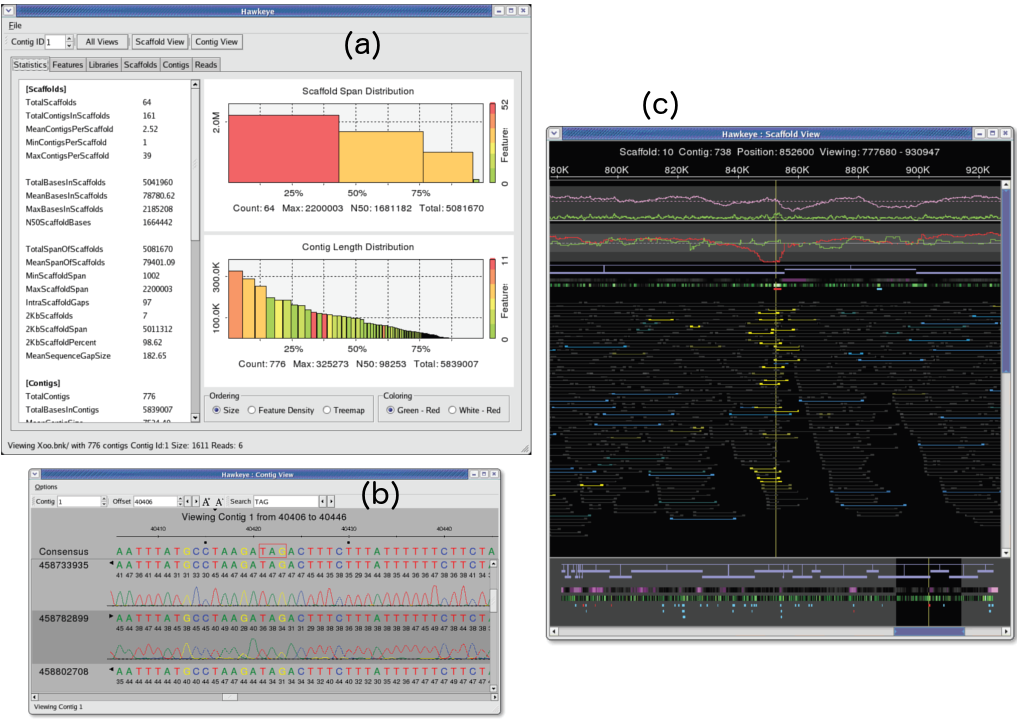
\includegraphics[height=5.7in,angle=90]{figures/hawkeye.png}
\caption[Hawkeye Interface Views.]{Snapshots of the available views in the Hawkeye tool: (a) Launch Pad, (b) Scaffold View and (c) Contig View.
\label{fig:hawkeye}}
\end{figure}

The formats to store read alignment information have been influenced by the technical changes imposed by the new technologies associated with NGS. The SAM format was created as part of the 1000 genomes project as an attempt to provide a generic alignment format that support single and paired reads. A SAM file is a text file that follow the SAM format, this file can then been converted to BAM, which is a binary lossless compressed file that can be indexed to offer rapid access to an specific position of the alignment \cite{HEN2009}. 

A set of tools called SAMtools was developed by the same team in order to help with the basic operations required to manipulate a SAM file. It includes a Text Alignment Viewer, which despite been very basic and command line based, is of great help to researchers because by been so basic makes the navigation on full genomes very fast.

Similar formats to SAM have been developed around the NGS technologies in order to store different types of data.  For instance, BigBed and BigWig, which  are the Big Binary Indexed (BBI) version of the BED and WIG formats. BED files are used for tables with a varying number of fields, where each line contains the felds for one record separated for white space. WIG files are used to associate a double value to each base, it is designed to compress information when the same value is assigned to a big section \cite{KEN2010}.

The Integrative Genomics Viewer IGV is one of the tools that take advantage of these new formats to enable real time exploration of large-scale genomic data-sets in different resolution scales \cite{ROB2011}. Data sets of both basic aligned read sets as well as deviated results can be loaded into IGV from local and remote sources. IGV can then be used to detect and correct assembly errors such as misalignments in repeat regions. IGV also supports the display of annotations files in context of the genome, making it suitable for the category (ii) defined at the beginning of this section.

A description of other tools that support the process of sequencing a genome (category (i)) can be found in \cite{NIE2010}. Once the genome is ready and has been through a finishing process it is usually shared and other scientist can use it in context of their own data. Is in this stage where the tools of category (ii) i.e. browsing a completed genome with its annotations; are of great help.

\subsubsection{Genome Browsing}
A famous principle in visualisation is known as the Shneiderman mantra: \emph{overview, zoom, filter, details-on-demand} \cite{SHN1996}. Most genome browsers use a similar layout that follows the mantra quite closely, adapting it to the molecular biology behind the data:

The \emph{overview} is usually a graphical representation of the karyotype, which is the set of chromosomes displaying its bands. The bands have been experimentally defined using some cytogenetics techniques to have visual mark on the chromosome, and serve the purpose of the visualisation to identify the different chromosomic regions.

The user can \emph{zoom} into a chromosome band, or can select a region of interest by interactively mark an area, or by explicitly introduce the coordinates. Once a region of interest (ROI) is selected, a multi-row visualization is displayed, where the first row represents the ROI, some browsers use colour coding for this row to show the limits of the bands or other high level features of that region.

Each subsequent row is called track and displays a different set of features drawn proportional to the selected region. For instance, it is common to include a track displaying the annotated genes in the ROI, representing boxes to delimit exons, and lines for intrones. Other symbols can be use to represent different features, e.g. arrows to define if the gene gets translated in the direction 5'UTR or the other way around, colours can be used to represent the functional class of the gene, etc.

Most genome browser have a wide list of sources that provide different type of information such as transcription factors, single nucleotide polymorphism SNP, details about the sequencing source (e.g. contains, reads), proteins, supporting evidence, etc. The tracks to include in the browser are then selected and \emph{filtered} by the user. 

Finally a feature of interest can be selected to obtain \emph{details-on-demand}, for instance, to get link to a website that contains the information of the protein that gets produced by the selected gene, or specific data on the allele frequency of a SNP and its associated phenotype.

\begin{figure}  
\centering
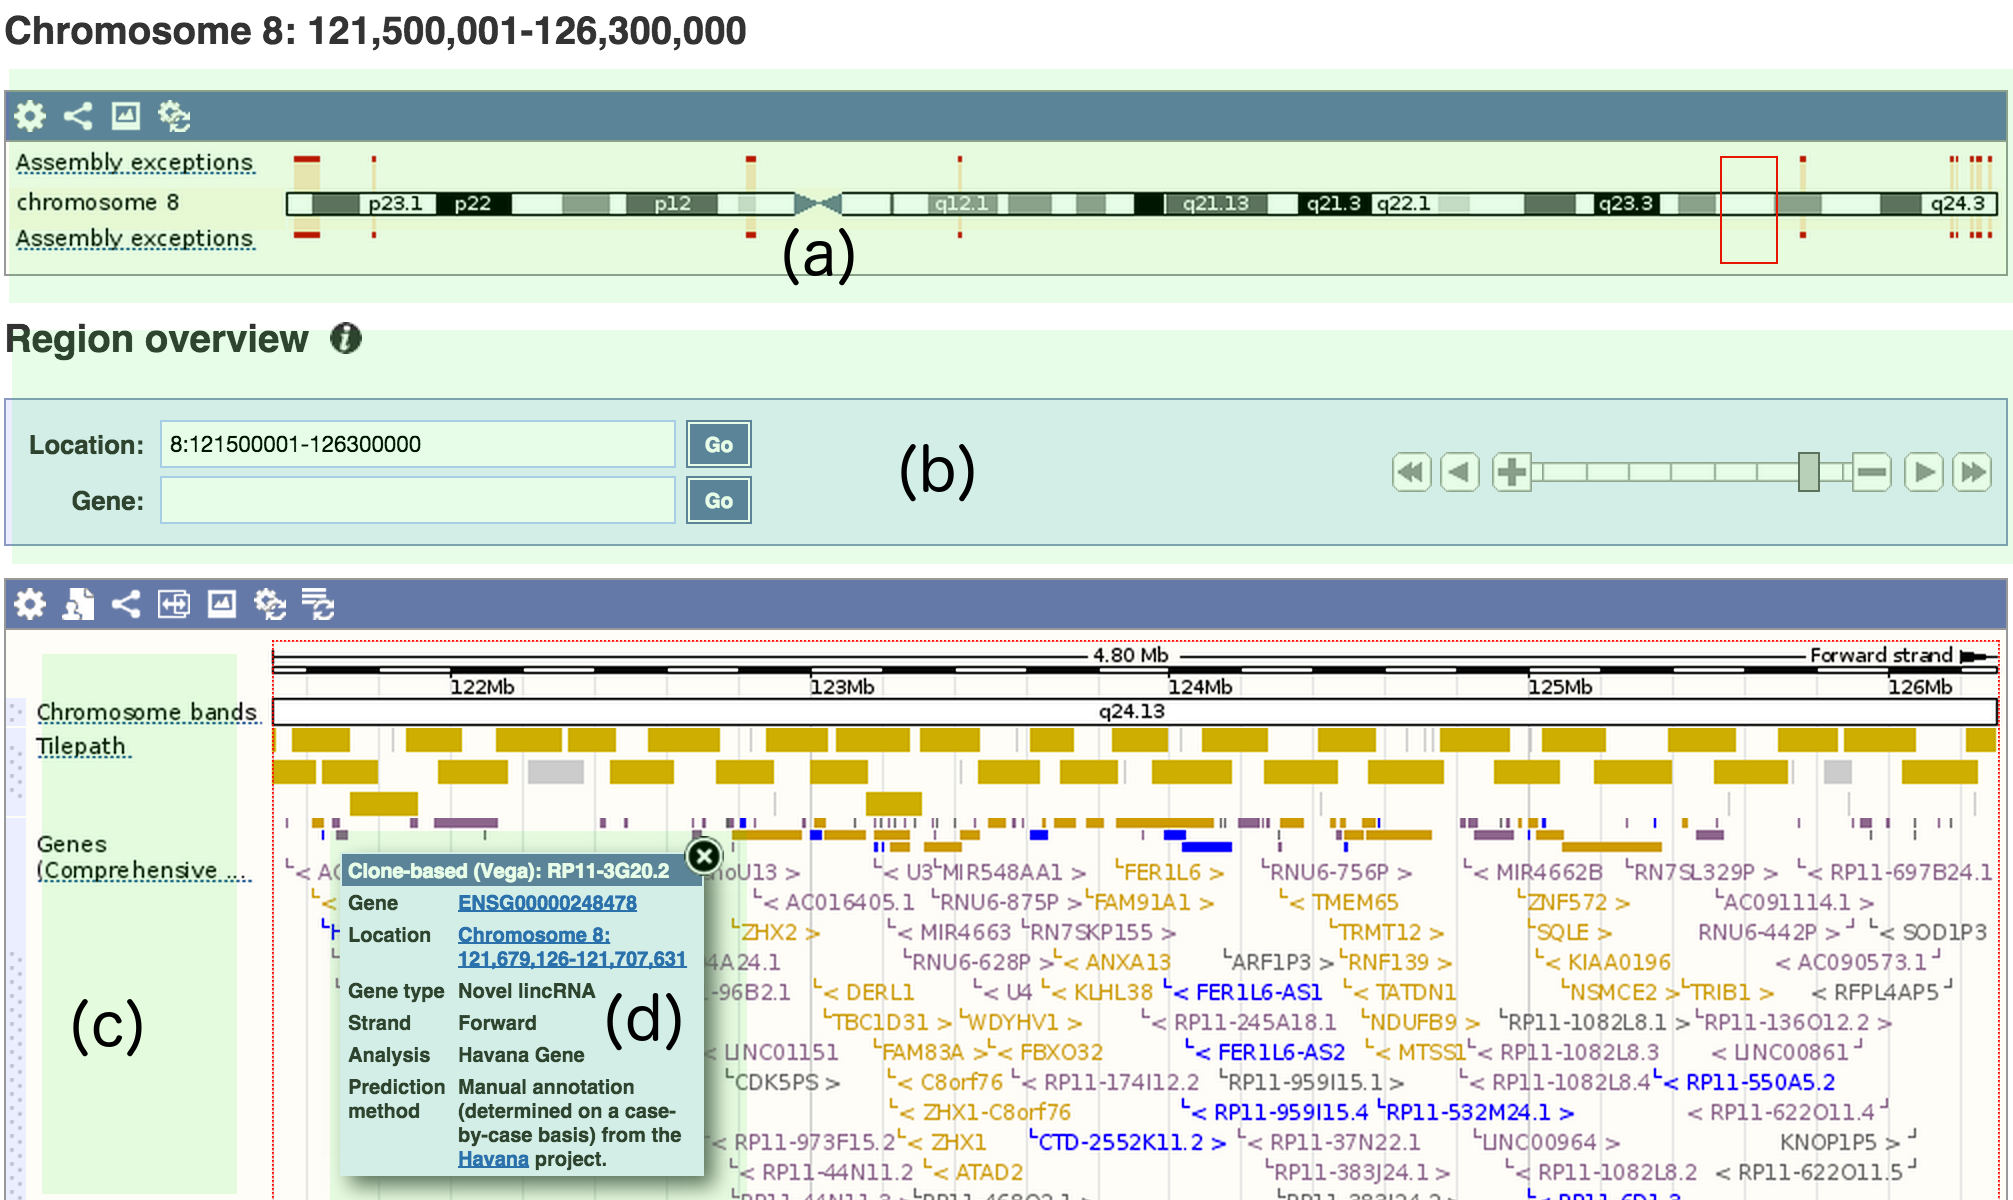
\includegraphics[width=\textwidth]{figures/ensembl_snapshot.png}
\caption[Snapshot of the Emsembl genome browser.]{Snapshot of the Emsembl genome browser highlighting the components that support the implementation of Shneiderman mantra: overview(a), zoom(b), filter(c), details-on-demand(d).
\label{fig:ensembl_sn}}
\end{figure}

Figure \ref{fig:ensembl_sn} shows some of the widgets used by the Ensembl genome browser, that follow the Shneiderman mantra. Region (a) displays a selected chromosome showing the overview of the data, in (b) it is possible to select the zoom level and the coordinates to mark the ROI; (c) show the name of the sources that have been selected for the current graphic, and (d) is a pop-up window shown when a click was done over one of the features of the graphic.

The Ensemble website (\url{http://www.ensembl.org/}) is only the window to see all the information that has been integrated through the Ensemble project. The dataset has grown from having partial information for human in 1999 to include full support to 69 species by the time of the release of version 77 in October 2014. 

From the beginning the objective of the Ensembl genome viewer was to support multiple species with a single software installation. The challenge goes further than the amount of data generated by species, because there are many differences in the data from one species to another \cite{STA2004}. The project has been clearly successful, not only judging by the number of species included, but more importantly for its big community, reflected by more than 1500 user queries assisted by their helpdesk team \cite{CUN2014}.

Besides the sources provided by Ensembl, it is possible to include external ones by using several protocols. For example, it is possible to include an URL to several NGS files (e.g. BAM, BigBed, etc.), or to point to an existing data source that uses the DAS protocol (discussed in section \ref{ssec:DASprotocol}); with this information Ensembl will query that source to get info in the ROI and display it in locations views, such as Region in detail, chromosome or karyotype. Moreover, Ensemble is in itself a DAS source, which makes easy the inclusion of its data in other resources \cite{SPU2010}.

Similar efforts to Ensembl have been addressed by two other big organizations: the NCBI Map Viewer \cite{ACL2014} and the UCSC Genome Browser \cite{ROS2014}. Both projects provide easy access to the centralised repositories of each institution, and allow to include third party access to be displayed in context of their data. Moreover, they collaborate with each other, and information from one source is available to be displayed in the other. A comparison between these three genome browsers can be found in \cite{FUR2006}.

These traditional genome browsers share the same architecture, where both data and service are located on the server side: When a new request gets to any of them, the data is collected form local or third-party data sources, and then, an image is generated in the server, and ultimately transmitted to the client; HTML link-maps are also generated to be able to use parts of the generated image as interactive links. In this way the client only requires to be able to display images and the use of the \emph{map} HTML element, which is part go the HTML specification since early versions, and therefore is widely supported.

Unfortunately by using this approach it is necessary to re-generate a completely new image with most user interactions, for example, by moving the ROI by a few bases, or by hiding a data source. Some strategies, have been creates to improve the usability of these applications, for instance using cache memory in the server to accelerate the access to remote sources, or pre generate the most likely required images (e.g. left and right of the current region). Nonetheless, factors such as the number of sources or network delays can affect dramatically the smoothness of the navigation in a system of this type.

Recent web technologies permit the decentralisation of the data, increasing the workload on the client and therefore liberating the server from most of the display related tasks. Under this model, the web genome browser is an application that mainly runs in the client, requesting data on-demand and generating/manipulating the graphic accordingly. If, for example, the user drags the display area to the right, making visible a few more bases, the client only requests the information of the new area and complement the graphic dynamically, reducing the computational cost of creating a full image, but most importantly isolating all the ``look and feel'' tasks from the server, allowing the server to focus on serving data, making it able to attend more and bigger requests.

JBrowse is an open source application that follows this approach implementing a robust client in JavaScript with the support of a server side developed in Perl for the preprocessing of the data. JBrowse uses a combination of standard HTML 'div' and 'canvas' elements to represent the genomic features. For instance in high level views of data, 'divs' are used to create histograms to show the amount of features in an area. As in the case of other genome browsers, JBrowse support the inclusion of third-party data using NGS files, for example BigWig data is represented either as heat maps or histograms using 'canvas' elements \cite{LEE2013}.

There is different strategy for genome browsing, which takes advantage of the features of what is also known as Rich Internet Applications RIA; the alternative is to preprocess the information to create small images called tiles that can be used to compose a view, similar to the experience introduced by Google maps; in this way there is no need to refresh a whole page if there are minor changes in the selected area. 

However, in \cite{SKI2009} the authors of JBrowse present a benchmarking experiment, where the two approaches are tested, showing better response times in the case of using HTML elements. Besides the performance, the 'tiles' approach requires a lot more storage space in order to have all the tiles pre-calculated, moreover, the approach complicates the desirable feature of including third-party sources because it might need to pre-process the entire source to create the tiles.

A similar project to JBrowse is Dalliance, a Web-based Genome Viewer developed using the HTML5 capabilities to manipulate SVG elements. It also requires a modern web browser (Firefox 3.6+, Chrome 5+, Safari+). Dalliance takes advantage of the DAS architecture in order to allow the users to put custom data in context of reference genomes. As other genome browsers mentioned above, it supports the interaction with BAM files and other NGS related formats \cite{DOW2011}. 

Similar use of DAS, has been implemented in MyKarioView (discussed further in section \ref{section:mykarioview}), which has an special emphasis on the display of personal genome data in context of well known data sources.

It is important to highlight that the purpose of genome browsers is to simplify the task of generating hypothesis based in the aggregation of genomic data. Each data source can contain errors, and the researcher should be sceptical of any conclusion based on a single observation. Genome browsers allow to graphically display several sources, and in this way make easier the detection of anomalies, errors or special genomic conditions. Despite how evident a hypothesis is represented in a visualisation, the scientist must have access to the original data in order to evaluate any theory \cite{CLI2009}.

\subsubsection{Comparative Genomics}
The last of the categories (iii) mentioned in the beginning of this section refers to the group of tools used to compare genomes in between individuals and/or species.

With the constantly growing number of complete genomes, it is only a logical step in research, to start looking for high level similarities between them and to use the discovered knowledge for one species in the research of others. This field, known as comparative genomics, tries to identify functional elements common in multiple species and their evolutionary modifications, but is also common to use these techniques in order to help in the assembly and finishing of new genomes.

The estimation of the conservation of the chromosomal location of multiple genes among several species is known as synteny. The relevance of it, is in the assumption that a sequence of genes on the same location in two species is a an indication of a common ancestor. A "dot plot" graphic (see Figure \ref{fig:dotplot}) is commonly used to represent the synteny among  2 genomes. Each of the 2 dimensional axis of the plot represent one of the genomes, and dots in the graph are the positions where a common gene is located; connected dots that show a 45 degree line, are the indication of a high syntenic region. Tools such Vista \cite{FRA2004} and GenomeMatcher \cite{OHT2008} include implementations of dot plots among other ways to compare genomes.

\begin{figure}  
\centering
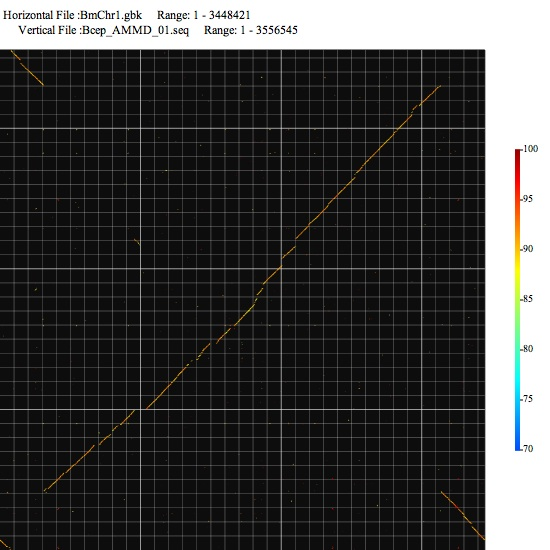
\includegraphics[width=4in]{figures/dotplot.jpg}
\caption[Dot plot comparison created with GenomeMatcher.]{Dot plot comparison created with GenomeMatcher
\label{fig:dotplot}}
\end{figure}

An alternative to dot plots, some tools offer a technique to display multiple genome alignments and marking corresponding areas in between by colour-shadowing, for example Figure \ref{fig:gbrowsesyn} shows an example generated using GBrowse\_syn \cite{MCK2010} where multiple genomes from the WormBase database have been aligned and a section of it is displayed to show the conservation certain genes.

\begin{figure}  
\centering
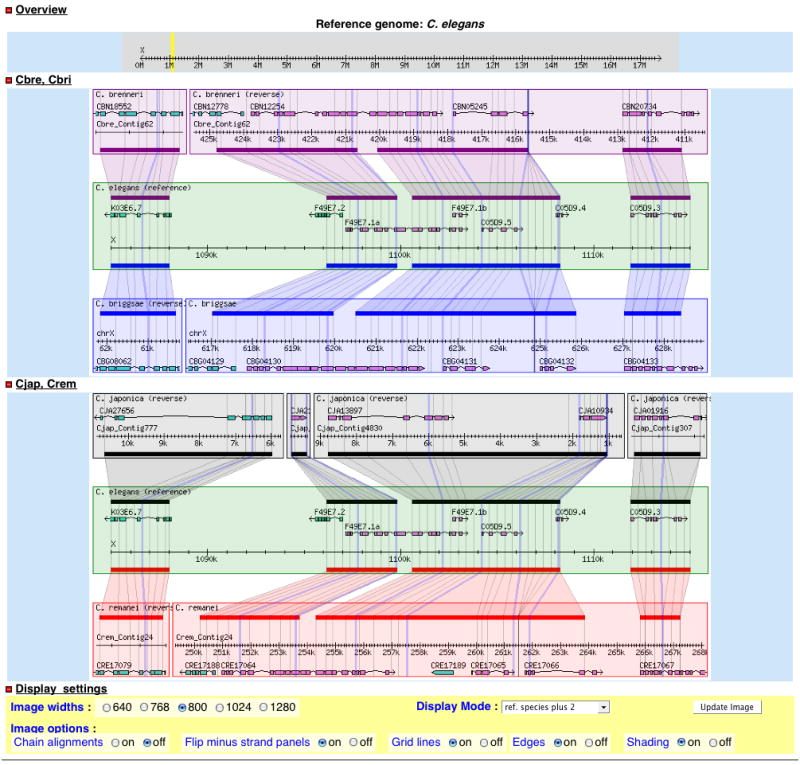
\includegraphics[width=\textwidth]{figures/gbrowse_syn.jpg}
\caption[multiple alignment snapshot generated with GBrowse\_syn.]{A five species whole genome DNA sequence alignment comparison from WormBase using GBrowse\_syn.
\label{fig:gbrowsesyn}}
\end{figure}

Besides the comparison of genomes in between species, the progress in the sequencing techniques permits the analysis of multiple individuals genomes in order to study their variation, and try to discover in this way the genotype that causes phenotypes of interest such as diseases. The biggest yet international effort in this area is known as the 1000 Genomes project,  which in their latest publication \cite{GEN2012} includes the genomes of 1092 individuals from 14 populations, and discovered and genotyped 38 million SNPs, 1.4 million indels and 14000 large deletions; vital information for genomic studies of human health.

An adaptation of the Ensembl browser has been develop in order to provide a way to visually browse over the result information of the 1000 Genomes project. Multiple tracks including aggregates and results from the study can be included in the browser and new tools to export and visualise variation data have been included.

\subsection{Proteomics}
In the central dogma of biology, DNA (deoxyribonucleic acid) encodes genes, which get transcribed in RNA (ribonucleic acid), which in turn, gets translated into proteins. Each of these is represented by a sequence of either nucleotides (DNA, RNA) or amino acids (Proteins). On the previous Section we discussed the visualisation tools that assist the process of sequencing DNA in order to get a full genome of an species, where positional annotations can be included, shared and explored, in the context of one or multiple organisms. 

It is because of the central dogma that annotations about genes are among the most used and useful features to know on a DNA sequence. The direct connection between a gene and a protein is the key to big part of the molecular biology research. For example, many diseases are caused because there are not enough (or too many) proteins to execute a biological function, or because there are proteins but they are malformed; in any of those cases the source of the problem can sometimes be trace back to the gene that generated that protein, and find that a mutation have appeared and a section of nucleotides have been inserted/deleted (indels). 

It is one of the goals of proteomics, at least in the clinical context, to deliver markers for disease prognosis, state and treatment outcome and targets for disease treatment \cite{MIS2007}. The Online Mendelian Inheritance in Man OMIM resource, is a catalog of human genes and genetic disorders \cite{AMB2014}. In OMIM is possible to find what mutation in a gene (genotype) is associated with a disease (phenotype). This information has been compiled from peer reviewed publications that represent the current knowledge in the area from several communities (clinicians, molecular biologists and genome scientists), this, of course is a work in continuos progress and despite the enormous contribution of resources such OMIM, it is not by any means, a finished task.

Once a good approximation of the genome of an organism has been identified, deciphering its proteome (i.e. the total protein complement of a cell, organ or even an organism) it is the logical step to follow, specially if considering that the number of identified genes during the human genome project (~30000) is way too small to explain the complexity of human biology \cite{PAN2008}.

%There are different experiments that look for clues in the role played by proteins in the different parts of this puzzle. 
This is due (among other reasons) to gene and protein splicing and post-translational modifications PMS, which then makes it impossible to completely deduce the proteome from the genome, therefore, approaches that start by the protein identification are necessary. Besides, the discovery of genes by computational means is limited and proteomics techniques offer an alternative.

Multiple experiments have been develop in order to approach this challenge, for example, mass spectrometry MS, helps to identify which peptides and ultimately which proteins are present in a given sample; 2D gel electrophoresis and microarrays analysis can give insights in the proportions of proteins that have been expressed in certain conditions (e.g. an specific tissue, a sick patient, a health person(control), etc.), similar data can now be obtained with alternative uses of NGS technologies such RNASeq; crystallography and modelling software has been used to find the final shape of the protein.

Visualisation has shown his potential by helping in the understanding and analysis of the outcomes of such experiments. Below we will show some cases grouped by some of the most used proteomics technique, where visualization methods have been used to support the analysis.

\subsubsection{Gel Based Proteomics}
Two-dimensional gel electrophoresis 2DE is still the most used approach in top-down proteomic studies mostly due to its efficiency at separating proteins in complex mixtures. Figure \ref{fig:gelflow} present the usual steps involved in an 2DE experiment that separates the proteins of interest for a particular hypothesis, which can be then identified with for example MS techniques \cite{SIL2014}.

The 4 first stages on this flow describe the preparation and execution of the experiment itself, which results on a set of gels (one per sample), where proteins are separated according to molecular size and isoelectric point. Conglomeration of proteins are then exposed as darker spots. In order to analyse the relevance of the different proteins on the hypothesis of the particular study, the gels need to be digitalised and processed, quantifying the protein concentration on each of the detected spots (alternatively some techniques quantify per pixel). Multiple techniques of image processing are applied in order to clean and extract the data; then normalisation and stabilisation is executed. The output of this process is a matrix in which every row represents a sample, and every column represents a spot across all gels; values in the matrix are then the level of concentration on an spot of a given sample. 

\begin{figure}  
\centering
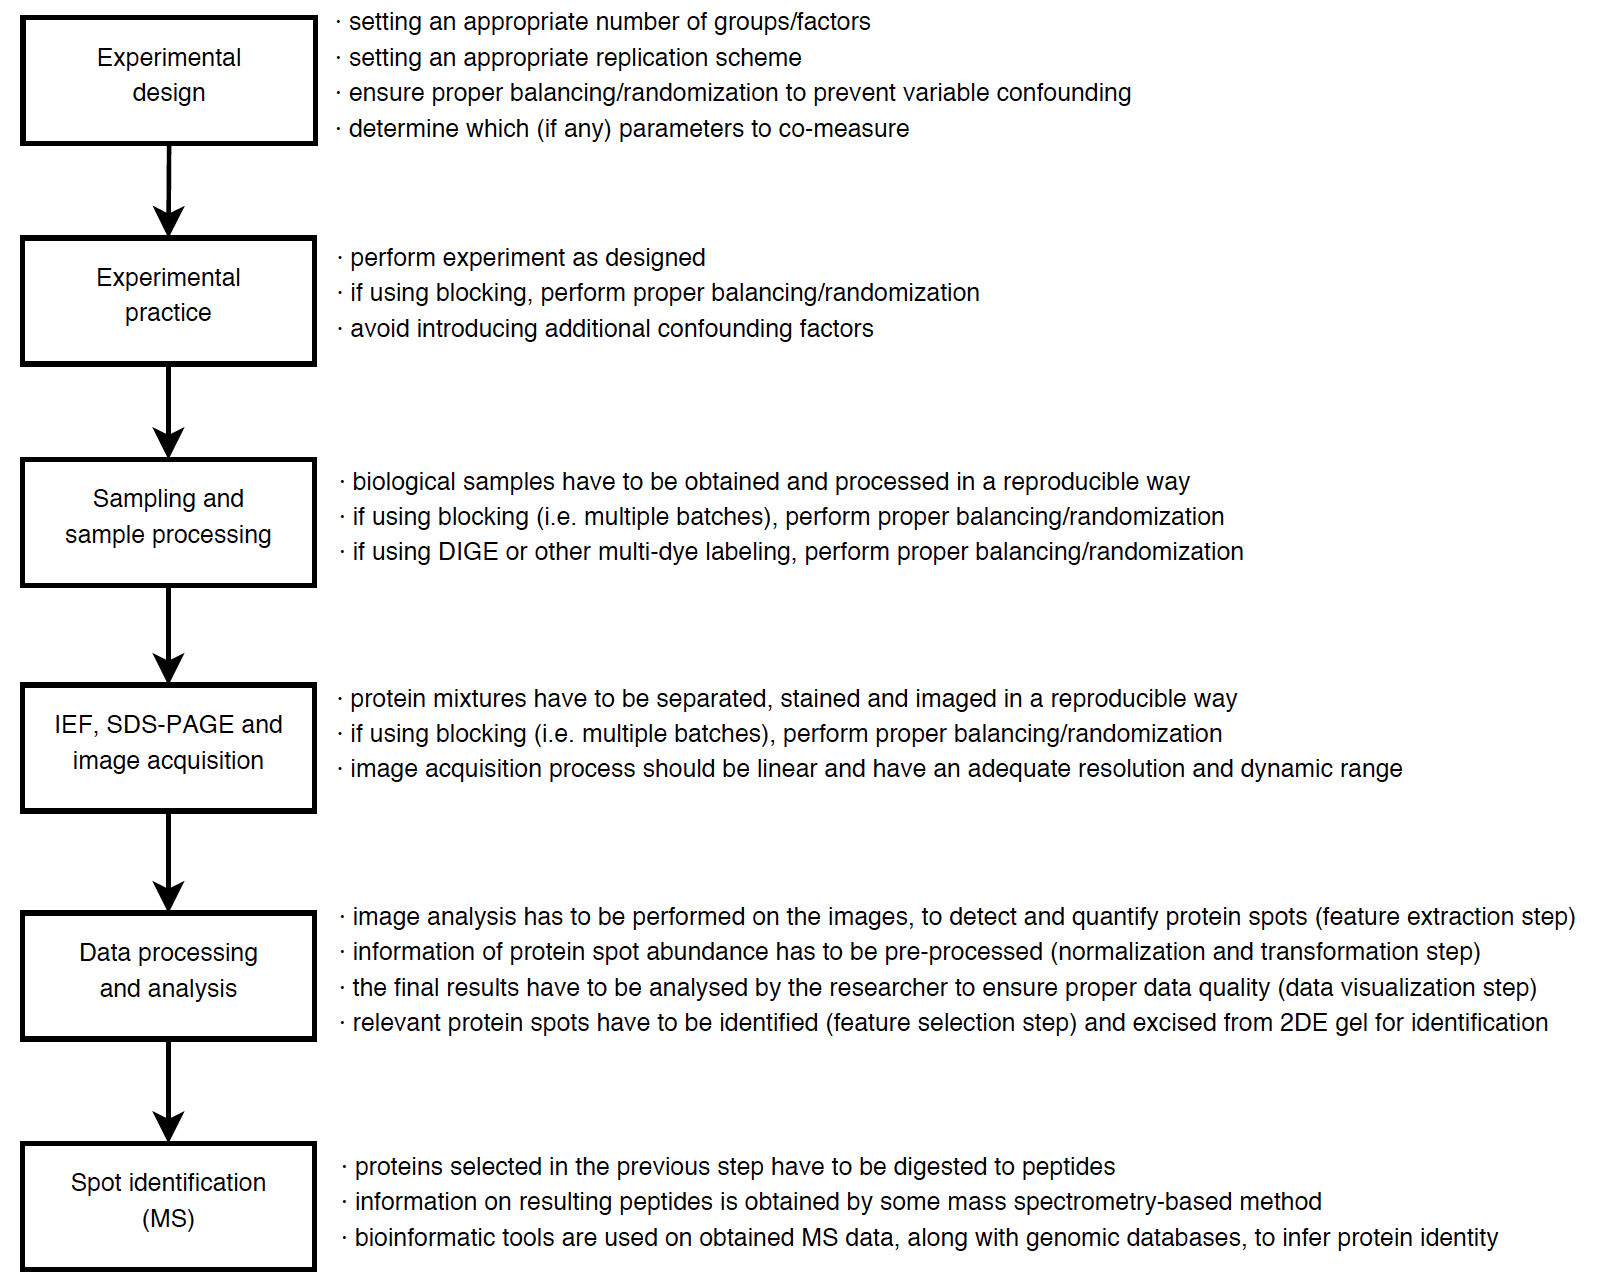
\includegraphics[width=\textwidth]{figures/gel-based.png}
\caption[High level overview of a typical gel based proteomics workflow.]{High level overview of a typical gel based proteomics workflow.
\label{fig:gelflow}}
\end{figure}

There are different protocols for gel-based experiments trying to overcome the different limitations of this technique (i.e. low resolution, low dynamic range, bias agains categories and low reproducibility), and the Differential Imaging Gel Electrophoresis DIGE, has become one of the best alternatives. The main difference of DIGE with other protocols is that control and case samples are tagged with different fluorescent dyes, which facilitates the spot detection and its posterior quantification \cite{PAN2008}.

In most of the protocols, each of the gels can have other variables associated, for instance, the tissue that it belongs to, information about the donor (e.g. sex, age, weight) and data about the hypothesis (e.g. healthy/infected). The relevance of a spot in the context of the study hypothesis and considering all the mentioned variables, it is used to filter the required protein identification experiments, and ultimately reduce time and costs to proof/disproof the hypothesis. It is in this step where statistical and visualisation techniques are of great help for the researcher.

The problem is that common visualisation techniques (e.g. box plots, scatter plots) are usually not enough, because the number of variables(spots) to include is too high(in the order of hundreds), and therefore multivariable techniques that combine statistical methods and visualisation tools are required at this stage.

Principal Components Analysis PCA has become the preferred technique in 2DE, because it offers a good and unbiased view of a dataset along the subspace where most variation occurs. PCA looks for a 2D or 3D representation of the data where the axis are the principal components PC (hence its name) that most highly contribute to determine the variance of the data. A PC is not a single variable but rather a projection of the combination of several ones, and the result of a PCA gives the contribution of each of the variables for each PC.

Figure \ref{fig:PCA} serves as an example of the visualisation of the results of a PCA on a data set in which 2 treatments (``A'' and ``B'') were been compared with biological samples being taken at three time-points: 0h, 6h and 48h; colour-coded as light grey, dark grey and black respectively. There is a clear division of 2 groups. In a 2DE experiment is common to select the spots to analyse further by studying the variable contribution on each PC.

\begin{figure}  
\centering
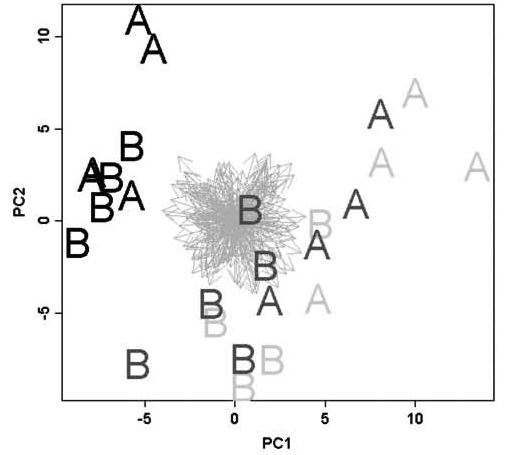
\includegraphics[width=4in]{figures/PCA.png}
\caption[Example of a PCA result plot.]{A biplot displaying PCA results 
\label{fig:PCA}}
\end{figure}

PCA uses the euclidean distance when calculating the projections of the variable contributions on each PC, this strategy has shown a good balance of outcome/performance for multidimensional data, however when the number of dimensions is really high it can be misleading, and then other techniques are  necessary, foe example, Independent Component Analysis ICA, Partial Least Squares PLS, Metrical multi-Dimensional Scaling MDS, Non-Metrical multi-Dimensional Scaling NMDS, clustering methods and Self-Organised Maps SOM. A discussion about this methods in 2DE can be found in \cite{SIL2014}.



\subsubsection{Mass Spectrometry Techniques}
Proteomics based on mass spectrometry it is about identifying, quantifying and characterising  as many proteins as possible in a single experiment . Probably the inflection point for the usage of MS techniques was the definition of the tandem mass spectrometry (also known as MS/MS) because it allows the identification of a large number of proteins on a high throughput manner .

A MS experiment it is commonly the the next step after getting the results of a separation process. In the case of 2DE, the spots are cut out of the gel, and the proteins are digested into shorter peptides by an enzyme and then separated in order to reduce the sample complexity and to get better performance out of the mass spectrometer.

The workflow to analyse the MS/MS results is described in figure \ref{fig:ms_workflow}. The input is the row data generated by the mass spectrometer, which format is usually native to the machine, and therefore the first step is to convert the files into more standard formats; the mass spectra datum of each peptide is used to try to identify it, which usually involves searching for similar mass spectra of known (or hypothetical) peptides; followed by a validation step; and then the inference of the target proteins is calculated; the following stages are included or not depending on the nature of the experiment (e.g. requires quantification because it is a comparison of control v.s. sample) or the setup of the laboratory (e.g. it uses a Laboratory Information Management System LIMS, or not). \cite{DEU2008} includes a more complete description of this workflow and the most well-known software tools associated with each step.

\begin{figure}  
\centering
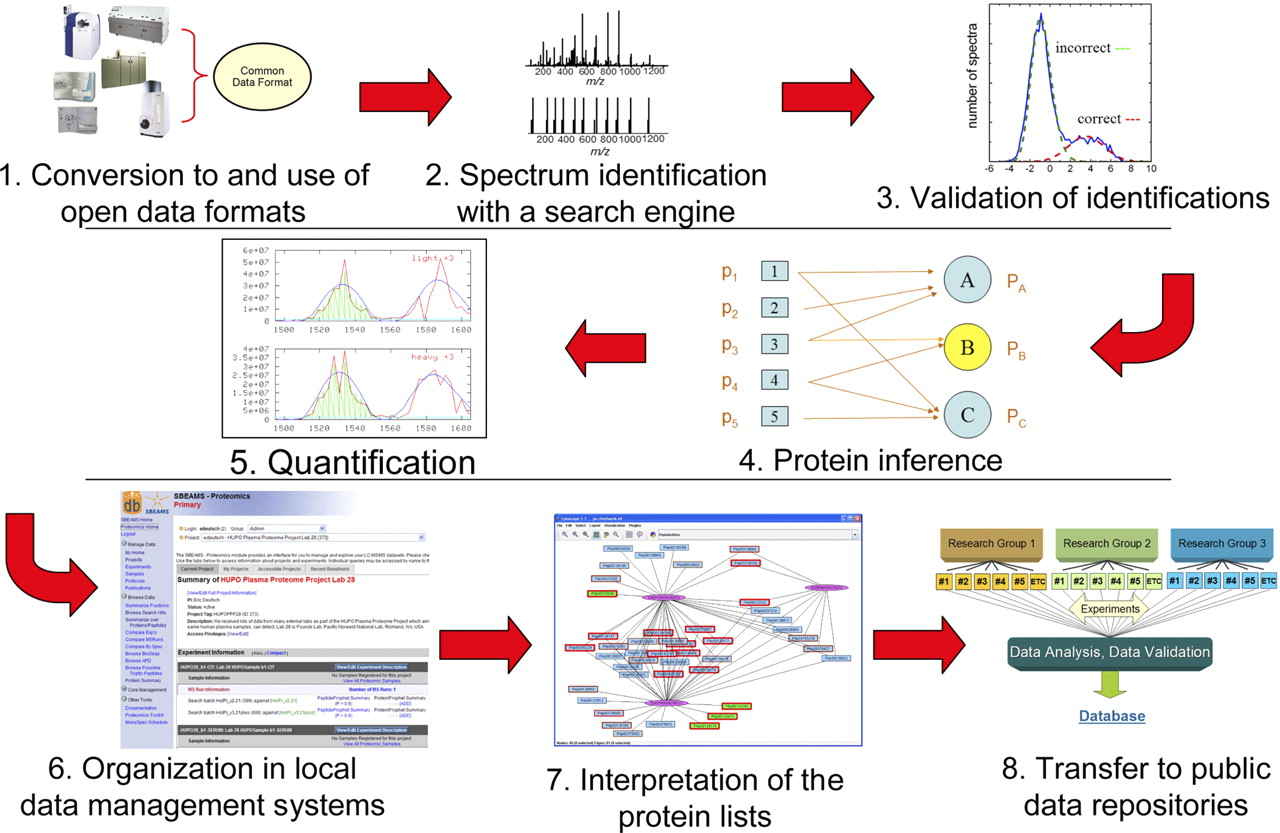
\includegraphics[width=6in]{figures/ms_workflow.png}
\caption[Tandem mass spectrometry workflow.]{Tandem mass spectrometry workflow
\label{fig:ms_workflow}}
\end{figure}


A classification of the most frequent tasks based on the described workflow have been included in \cite{PER2014} in order to describe the contributions of different open source libraries in MS experiments. Below we describe the two software tools mentioned there that include several visualisation techniques to aid in the different stages of the MS workflow. An extended list of visualization tools in MS/MS based proteomics can be found in the section 5 of \cite{JAC2010}.

\paragraph{PRIDE Inspector}
The PRoteomics IDEntifications database PRIDE, is a centralised repository where proteomics data is stored and shared. In order to submit data into PRIDE a series of standards have to be followed. This with the purpose of ensuring a good quality level of  the data. This type of resources have been used more often in part because some journals recommend the use of data standards and to be shared in public repositories; in some cases those are necessary conditions to the publication of the article.

PRIDE Converter  (\url{https://code.google.com/p/pride-converter/}) is a tool that gives support on the process to submit new data to PRIDE. The same team developed PRIDE Inspector, following the success of the converter, and motivated by the fact that inspection and validation of reported results are of great importance during the review process \cite{WAN2012}.

\begin{figure}  
\centering
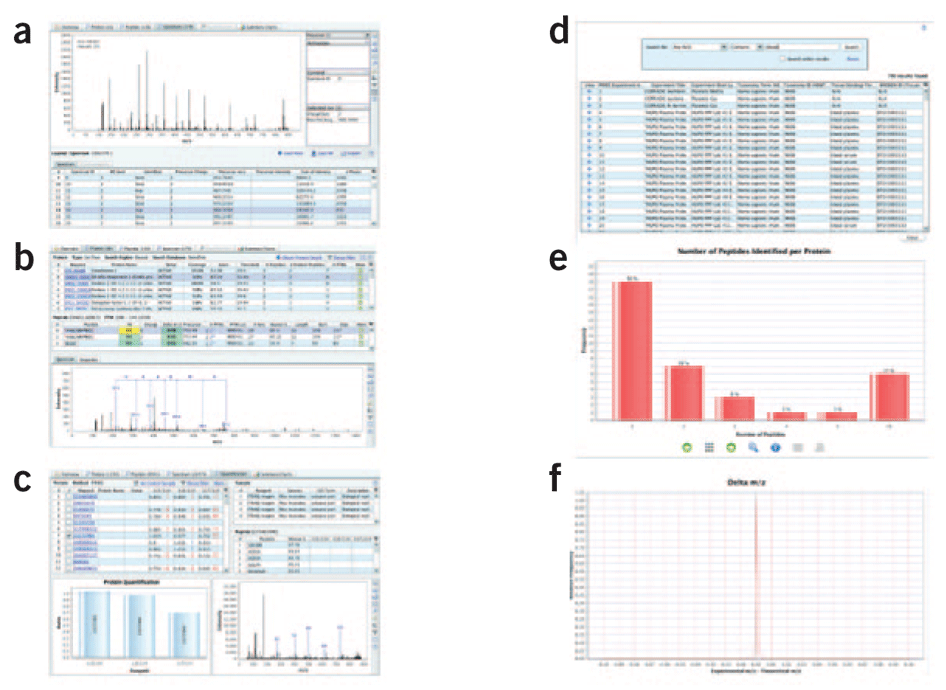
\includegraphics[width=\textwidth]{figures/prideinspector.png}
\caption[Views on the PRIDE inspector toolset.]{(a) Section of the spectrum view tab. (b) Protein view tab, including the spectrum viewer showing MS/MS fragment ion annotations (only b ion annotations are shown). (c) Quantification view. (d) 'Search PRIDE' panel. (e) Number of peptides identified per protein chart. (f) 'Delta m/z' chart.
\label{fig:pride}}
\end{figure}

Figure \ref{fig:pride} is a group of some of the views of the PRIDE Inspector application. To start with PRIDE Inspector the user can load their own data or explore the public data from PRIDE using the search view(d); the proteins of the data set are listed (b) including its peptides, PTMs and corresponding spectra; the spectrum viewer (a) includes automatic annotations based on submitted fragmentations; some aggregate charts (e) and (f) are also  available to explore the information of each protein; and if the experiment includes quantification data, the view in (e) is enabled and the data can then be used to create comparative charts.

PRIDE Inspector was developed with modularity in mind, and as a consequence, libraries packaging some of the functionalities can be obtained independently. The visualisation routines are accessible from a library called mzGraph that can be reuse in other projects.

\paragraph{Rover}
The open source Java application called Rover, focuses in quantitative proteomics data, it generates visualisations of this data that help the user in the process of selecting and validating  algorithm suggested regulated proteins in the context of a whole experiments \cite{PER2014}.

Quantitive proteomics datasets are composed of two parts on Rover: peptide identifications and quantitative data. Rover includes a wizard-like menu that facilitates the input of these files; it also includes several parsers for some of the most used formats of that type of data.

\begin{figure}  
\centering
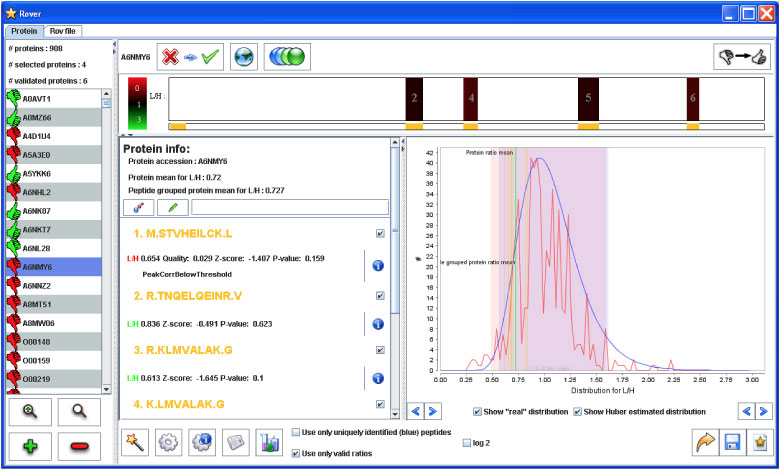
\includegraphics[width=\textwidth]{figures/rover.png}
\caption[The main Rover interface.]{The main Rover interface.
\label{fig:rover}}
\end{figure}

Once the data has been successfully loaded into Rover a high level view of it is presented to the user, so the user can select and validate the regulated proteins. 

Figure \ref{fig:rover} is an snapshot of the main interface of Rover, here it displays protein and peptide informations as follows: In the left side there is a panel displaying all the proteins part of the experiments, in which is indicated via glyphs if the protein is selected(thumbs up) or not(thumbs up), and colour coded if is validated(green) or not validated(red). The top of the screen is the protein bar, where the peptides are drawn proportionally over a rectangle that represents the whole protein; and the centre of the window is then divided again, were the left side offers general information of the selected proteins and the right side displays the ratio distribution graph, where selected protein and partied ratios are shown in comparison with the reference set, using either the intrinsic distribution of the data or transforming the data to use the Huber distribution, which can give a new perspective to the analysed data \cite{COL2010}.

All generated data in Rover can be exported for posterior analysis.

\subsubsection{Micro Arrays}
Although Microarrays techniques are considered by some, out of the proteomics field because it deals with transcription data, more often than with proteins themselves; this technology offers a high throughput solution to study the expression levels of genes on a particular sample, which is expected to be proportional to the number of proteins that ultimately get produced. There have been advances in microarray techniques that use proteins in order to complement MS studies \cite{PRA2014}. Because of its high usage we will focus on visualisation tools used in the analysis of DNA/RNA microarrays, particularly we will describe 2 suites that serve to exemplify the most common scenarios where visualisation techniques applied to microarray data, this however is just an small sample of all the tools that are used to analyse this type of data.

\paragraph{Bioconductor}
Bioconductor is a library for the programming language R, that aims to bring support for general research in computational biology, but have orientated their efforts towards the statistical analysis of microarray experiment's data, covering many of the usual task required: preprocessing, quality control, normalisation and downstream inference of biological and clinical questions \cite{GEN2004}.

The development of Bioconductor has been inspired by the achievements of other software that follow the principles of the Free Software Foundation. The authors consider that the adaptation of these principles into the computational biology and bioinformatics fields, is key in order to improve research in terms of transparency (i.e. exposure of the entire process), reproducibility and efficiency of development.

R is a programming language recognised by its great numerical and statistical capabilities, which can be easily connected to many types of visualisation graphs. R can be used for rapid prototyping and quick exploration of data, it supports multiple network and parallel computing protocols, as well as access to different database systems. These reasons attracted the Bioconductor community when they were choosing which language to use in order to implement their goals.

The Bioconductor project has invested a lot of its time into the creation of the infrastructure of the project, for example, by defining protocols to the addition of new packages and its documentation, interfaces to the existing packages, documentation for both user and developer, exposure to the documentation from within the system, guidelines on how to use their source code repository, definition of good practices when developing a Bioconductor package, etc.

Thanks to all these efforts Bioconductor no has a strong community of users with more than 3000 subscribers to their forum and over one million visitors in their website, in which is possible to find over 800 software packages (release 2.14). Their publication \cite{GEN2004}. has more than 6000 citations and many of the packages developd for Bioconductor have been published in peer-reviewed journals as well \cite{BIO2014}.


\begin{figure}  
\centering
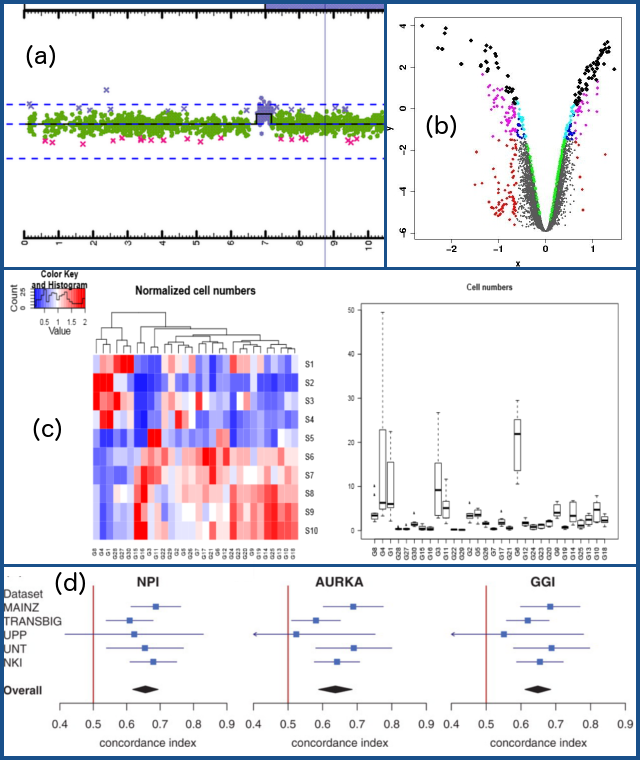
\includegraphics[width=\textwidth]{figures/bioconductor.png}
\caption[Visualisations created with Bioconductor's packages.]{Visualisations created with Bioconductor's packages: (a) aroma. (b) arrayQuality. (c) flowCyBar. (d) survcomp.
\label{fig:bioconductor}}
\end{figure}

In terms of visualisation the Bioconductor repository listed 218 packages with the tag visualisation by January 2015 (\url{http://www.bioconductor.org/packages/release/BiocViews.html#___Visualization}). Figure {fig:bioconductor} is a random selection of snapshots from several packages found in that list, in order to exemplify the wide scope of analysis and visualisations include in Bioconductor: (a) Aroma (\url{http://www.aroma-project.org/screenshots/}) provides a view similar to the on for genome browsers in order to display copy-number amplification in a chromosome; (b) is a diagnostic plot generated by arrayQuality \url{http://arrays.ucsf.edu/}; (c) is a clustered heat map and box plot, which result of an analysis of cell abundance changes in subcommunities deployed by using flowCyBar\url{http://www.ufz.de/index.php?de=32737}; and (d) is part of the case study used to exemplify survcomp \url{http://www.pmgenomics.ca/bhklab/software/survcomp} a package created to compare the performance of survival/risk prediction models. 


\paragraph{Chipster}
Chipster is a software suite that includes many of the most used software tools for the analysis and visualisation of microarray data and other high throughput experiments. It has a client-server architecture where the client is a graphical oriented interface that allows not only the display, but the interaction with visualisations; the server on the other hand is oriented to the execution and administration of the tools that a particular Chipster installation offers.

Cipster extensevely support the bioconductor package, allowing the edition of scripts to include the functionalities from the R package. Other tools can also be imported to Chipster, however only the ones written in bioconductor can be edited through Chipster.

Chipster is an exploratory tool were different tools and visualisation can be used at any time guided by the user's will. Moreover the execution history is saved as a workflow, and therefore it is easy to execute again with different data or tuning of the different tool's parameters. The workflow files can also be saved and shared.

There are more than 25 visualizations included in Chipster, the ones generated for the client software can be manipulated by the user, and also they serve as a way to interact, select and filter the data. The visualisation generated by Bioconductor and other imported tools are treated as static images and basic zooming and panning is supported. The interactive visualisation include scatter plots, volcano plots, venn diagrams, heat maps, self organised maps, among others; and can be used in different stages of a microarray experiment, e.g. normalisation, quality control, filtering, statistical testing, clustering, annotation, etc. \cite{KAL2011}.	


%Dasty, Interpro
\subsection{Protein Interactions}
%\subsection{Biological Pathways}
%\subsection{Population Variation}
%\subsubsection{General Research}
%To talk about statistical graphs and things like heat maps, phylogenetic trees, etc.

\subsection{Discussion}
Genome Browsers have evolve from simple displays of genes and transcripts to visual integration tools of biological data.

The spectrum of visualisation techniques in bioinformatics goes from simple 2 dimensional plots used to display elaborated statistics such PCA, to elaborated visualisation tools to display data which only preprocessing is scaling. 

%\section{Thesis outline}
